\documentclass[a4paper,12pt]{report}
\usepackage{iftex}
\ifPDFTeX
\usepackage[T1]{fontenc}
\usepackage[utf8]{inputenc}
\else
\usepackage{fontspec} % Handles fonts in XeLaTeX. Replaces inputenc and fontenc.
\fi
\usepackage{geometry}
\geometry{margin=1in}
\usepackage{graphicx}
\usepackage[colorlinks=true, linkcolor=blue, citecolor=blue]{hyperref} % Made links active
\usepackage{titlesec}
\usepackage{setspace}
\usepackage{wrapfig}
\usepackage{subcaption} % Modern replacement for 'subfigure'
\usepackage{listings}
\usepackage{xcolor}
\usepackage{csquotes}
\usepackage{ragged2e}
\usepackage{lipsum}
\usepackage{pdfpages}
\usepackage{amsmath}
\usepackage{amssymb} % For math symbols
\usepackage{tocloft}
\usepackage{cite}
\usepackage{float}
\usepackage{bibentry}
\usepackage{multirow}
\usepackage{enumitem}
\usepackage{fancyhdr}
\usepackage{comment}
\usepackage{tabularx}
\usepackage{booktabs}
\usepackage{makecell}% provides \makecell
\usepackage{array}% for >{\raggedright\arraybackslash}X

% Define a centered column type 'C' used in `pos.tex` tables
\newcolumntype{C}[1]{>{\centering\arraybackslash}p{#1}}

% --- Customizations for ToC, LoF, LoT (Remove dot leaders) ---
\renewcommand{\cftchapleader}{\hfil} % Removes dots for chapters in ToC
\renewcommand{\cftsecleader}{\hfil}% Removes dots for sections in ToC
\renewcommand{\cftsubsecleader}{\hfil}% Removes dots for subsections in ToC
\renewcommand{\cftfigleader}{\hfil}% Removes dots for figures in LoF
\renewcommand{\cfttableader}{\hfil}% Removes dots for tables in LoT

% Keep your existing ToC/LoF customizations
\renewcommand{\cfttoctitlefont}{\centering\Huge\bfseries\color{blue}}
\renewcommand{\cftsecfont}{\normalfont}
\renewcommand{\cftsubsecfont}{\normalfont}
\renewcommand{\cftsubsubsecfont}{\normalfont}
\setlength{\cftbeforetoctitleskip}{0pt}
\setlength{\cftbeforesubsecskip}{0pt}

% For the list of figures
\renewcommand{\listfigurename}{List of Figures}
\renewcommand{\cftloftitlefont}{\centering\Large\bfseries\color{blue}}

% For the list of tables (add this if you haven't already)
\renewcommand{\listtablename}{List of Tables}
\renewcommand{\cftlottitlefont}{\centering\Large\bfseries\color{blue}}
% --- End Customizations ---

% --- NEW: Replicating your manual chapter/section style ---
% This makes \chapter{} look like your manual formatting
\titleformat{\chapter}[display]
{\normalfont\Large\bfseries\centering} % Format for the whole block
{\chaptertitlename\ \thechapter} % "CHAPTER X"
{0.2cm} % Space between "CHAPTER X" and title
{\Large\textbf} % Format for the title text
\titlespacing*{\chapter}{0pt}{0pt}{0.5cm} % left, before, after

% This makes \section{} look like your manual formatting
\titleformat{\section}
{\normalfont\fontsize{14pt}{12pt}\selectfont\bfseries} % Format
{\thesection} % Number (e.g., "4.1")
{1em} % Space after number
{} % Code before title

% This makes \subsection{} look like your manual formatting
\titleformat{\subsection}
{\normalfont\fontsize{13pt}{12pt}\selectfont\bfseries} % Format
{\thesubsection} % Number (e.g., "2.1.1")
{1em} % Space after number
{} % Code before title
% --- END OF NEW FORMATTING ---

% --- ADDED: Remove paragraph indentation globally ---
\setlength{\parindent}{0pt}
% ---

\begin{document}
\begin{center}
    \Large\textbf{{\textbf{VCAN: A MULTIPLE CANCER RISK
PREDICTION AI AGENT USING LLM FINE TUNING\\
}}}
\end{center}
\vspace{.1cm}
\begin{center}
        {\large {A MAIN PROJECT REPORT} \\[0.4cm]
    Submitted by \\[0.3cm]
    \begin{center}
    \begin{tabular}{l}
        \textbf{\large ALAN THOMAS (MBC22CS015)} \\
        \textbf{\large MATHEWS VINOY (MBC22CS047)} \\
        \textbf{\large SANDESH V ANTONY (MBC22CS058)} \\
        \textbf{\large SIRIL T NINAN (MBC22CS061)}
    \end{tabular}
\end{center}
    
        
       
   
    
    to\\[0.3cm]
    APJ Abdul Kalam Technological University \\[0.3cm]
    In partial fulfillment of requirements for the award of the degree \\[0.5cm]
    of\\[0.3cm]
    {\Large {Bachelor of Technology }} \\[0.1cm]
    in \\
    {\Large \textit{Computer Science and Engineering}} \\[0.5cm]
    }
    
\end{center}


\vspace{0.6cm}
\begin{figure}[h]
    \centering
    
\includegraphics[width=0.3\textwidth]{MBC.jpg}
\end{figure}
\vspace{0.6cm}
\begin{center}
\noindent\mbox{{\textbf{DEPARTMENT OF COMPUTER SCIENCE AND ENGINEERING}}} \\[0.1cm]
{\textbf{\small{MAR BASELIOS CHRISTIAN COLLEGE OF ENGINEERING AND TECHNOLOGY, PEERMADE}}} \\[0.5cm]
{\textbf{APRIL 2026}}
\end{center}

\thispagestyle{empty}
\vspace{2cm}
\begin{center}
\noindent \mbox{{\textbf{DEPARTMENT OF COMPUTER SCIENCE AND ENGINEERING}}} \\[0.4cm]
\textbf {\small MAR BASELIOS CHRISTIAN COLLEGE OF ENGINEERING AND TECHNOLOGY} \\[0.4cm]
\textbf{2025-2026}
\end{center}
\vspace{0.5cm}
\begin{figure}[h]
    \centering
    
\includegraphics[width=0.3\textwidth]{MBC.jpg}
\end{figure}

\begin{center}
    \Large\textbf{CERTIFICATE}
\end{center}

%\addcontentsline{toc}{chapter}{\numberline{}Abstract}%
\vspace{1cm}

\fontsize{12pt}{18pt}\selectfont
% Use the justify environment from ragged2e for reliable full justification.
% Allow a bit of emergency stretch so long words/names can break more gracefully.
% Use a full-width minipage so justification is measured against \textwidth reliably.
\begingroup
\emergencystretch=1em
\begin{minipage}{\textwidth}
\justifying
\noindent This is to certify that this report entitled \textbf{\enquote {VCAN: A MULTIPLE CANCER
RISK PREDICTION AI AGENT USING LLM FINE TUNING}} submitted by \textbf{ALAN THOMAS\allowbreak\ (MBC22CS015)}, \textbf{MATHEWS VINOY\allowbreak\ (MBC22CS047)}, \textbf{SANDESH V ANTONY \allowbreak\ (MBC22CS058)}, \textbf{SIRIL T NINAN\allowbreak\ (MBC22CS061)}, and to the APJ Abdul Kalam Technological University in partial fulfillment of the requirements for the award of the degree of B.Tech. in Computer Science and Engineering, is a bonafide report of the project work carried out by them under the guidance and supervision of \textbf{Dr. Ushus Maria Joseph}, Associate Professor, Department of Computer Science and Engineering. This report in any form has not been submitted to any other University or Institute for any purpose.
\end{minipage}
\endgroup
\par

\vspace{2cm} % Space before signatures

% Use minipages to create two blocks and \hfill to push them apart
\noindent % Prevent indentation

\begin{minipage}[t]{0.45\textwidth} 
    \raggedright % Forces left alignment within this block
    \textcolor{red}{\textbf{Dr. Ushus Maria Joseph}} \\
    Project Guide \\
    Associate Professor \\
    Department of CSE
\end{minipage}
\hfill % Pushes the second block to the far right
\begin{minipage}[t]{0.45\textwidth} 
    \raggedright % Forces left alignment within this block
    \textcolor{red}{\textbf{Dr. Ushus Maria Joseph}} \\
    Head of the Department \\
    Associate Professor \\
    Department of CSE
\end{minipage}



\thispagestyle{empty}



\thispagestyle{empty}

% --- CORRECTED FRONT MATTER ---
\pagenumbering{roman} % Start roman numerals
\vspace{2cm}

% --- Abstract and Acknowledgement are correct ---
\chapter*{DECLARATION}

\vspace{1cm}

\fontsize{12pt}{18pt}\selectfont
We hereby declare that this report entitled \textbf{\enquote {VCAN: A MULTIPLE CANCER RISK PREDICTION AI
AGENT USING LLM FINE TUNING}} is a bonafide record of the preliminary project work carried out by us under the supervision 
of \textbf{Dr. Ushus Maria Joseph} in the Department of Computer Science and Engineering Mar Baselios Christian College of Engineering and Technology, Peermade.The project proposal presented in this report have been presented for the award of any other degrees.\\
\\
Peermade \\
\\
Date: 1 April 2026 \\
\\
\\
\\
\\
\begin{spacing}{1}
	
	\begin{table}[h!]
		\centering
		\begin{tabular}{p{0.5cm} p{6cm} p{10cm}}
             \textbf{} &&\textbf {ALAN THOMAS(MBC22CS015)} \\[0.2cm]
            \textbf{} &&\textbf {MATHEWS VINOY(MBC22CS047)} \\[0.2cm]
            \textbf{} &&\textbf {SANDESH V ANTONY(MBC22CS058)} \\[0.2cm]
            \textbf{} && \textbf{SIRIL T NINAN(MBC22CS061)} \\[0.2cm]
            
			
		\end{tabular}
	\end{table}
\end{spacing}
\newpage

\chapter*{ACKNOWLEDGEMENT}
\addcontentsline{toc}{chapter}{\textit{Acknowledgement}} % This adds it to the ToC
\vspace{1cm}

\fontsize{12pt}{18pt}\selectfont


The success of this project was made possible through the guidance and support of many. We
are grateful to the Management of Mar Baselios Christian College of Engineering and Technology for the opportunity and platform to complete this work. Special thanks to our
Principal, \textbf{Dr.V I George, Principal}, for his exceptional support and the facilities provided. We deeply appreciate the supervision and assistance we received, which were crucial to the project's completion. \\
\\
We are extremely indebted to our Head of the Department, \textbf{Dr. Ushus Maria Joseph}, Associate Professor Department of Computer Science and Engineering, for her valuable suggestions and encouragement during the course of our project work. \\
\\
We are grateful to thank our project coordinator, \textbf{Prof. Aryalakshmi R}, Assistant Professor, Department of Computer Science and Engineering for her valuable support. \\
\\
We are deeply grateful to our project guide, \textbf{Dr. Ushus Maria Joseph}, Associate Professor, Department of Computer Science and Engineering, for her keen interest and guidance throughout our project, providing essential information for a successful presentation. We also appreciate the constant encouragement, support, and guidance from all the faculty members of the Department of Computer Science and Engineering, which were instrumental in completing our project work successfully. \\

\vspace{1cm}

\begin{spacing}{1}
	
	\begin{table}[h!]
		\centering
		\begin{tabular}{p{0.5cm} p{6cm} p{10cm}}
           \textbf{} &&\textbf {ALAN THOMAS(MBC22CS015)} \\[0.2cm]
            \textbf{} &&\textbf {MATHEWS VINOY(MBC22CS047)} \\[0.2cm]
            \textbf{} &&\textbf {SANDESH V ANTONY(MBC22CS058)} \\[0.2cm]
            \textbf{} && \textbf{SIRIL T NINAN(MBC22CS061)} \\[0.2cm]
		\end{tabular}
	\end{table}
\end{spacing}
\newpage

% Use the 'C' column type (defined in main.tex) for centered fixed-width columns.
%\providecommand{\Ccol}[1]{p{#1}} % removed: use C{<width>} instead
 
%---------------------po,psco-stuffs-----------------
\newpage
\begin{center}
    \textbf{\underline{COLLEGE VISION \& MISSION}}
\end{center}
\vspace{0.5cm}

\noindent \textbf{VISION} \\[0.2cm]
An Engineering Institute with global quality to groom competent engineers equipped to address the changing needs of society.
\vspace{0.5cm}

\noindent \textbf{MISSION} \\[0.2cm]
Our efforts are dedicated for developing a learner centric education environment to:
\begin{enumerate}
    \item Provide value-based technical learning
    \item Practice real world problem solving
    \item Foster team work in engineering design
    \item Inspire innovations and R\&D
\end{enumerate}
\vspace{1cm}

\begin{center}
    \textbf{\underline{DEPARTMENT VISION \& MISSION}}
\end{center}
\vspace{0.5cm}

\noindent \textbf{VISION} \\[0.2cm]
To become an excellent department by empowering the graduates to address the challenges in the fast-changing scenario, adhering to ethical values.
\vspace{0.5cm}

\noindent \textbf{MISSION} \\[0.2cm]
\begin{enumerate}
    \item Inculcate skills to solve complex engineering problems and instill entrepreneurial capabilities.
    \item Equip the students to advance with the recent trends and technology through Research and Innovations in the field of computer science.
    \item Facilitate the development of professional behavior, ethical values and the spirit of service to the society.
\end{enumerate}


% --- PAGE 2 ---
\newpage
% --- PROGRAMME EDUCATIONAL OBJECTIVES ---
\begin{center}
    \textbf{\underline{PROGRAMME EDUCATIONAL OBJECTIVES (PEOs)}}
\end{center}
\vspace{0.5cm}

\noindent \textbf{Our Graduates will be able to:}
\begin{itemize}[leftmargin=2.5cm]
    \item[\textbf{PEO1:}] Think creatively and critically to solve problems in a global context with varying complexity.
    \item[\textbf{PEO2:}] Exhibit leadership qualities, Ethical Values, managerial and entrepreneurship skills.
    \item[\textbf{PEO3:}] Contribute inventions and innovative advancements in information technology through life-long learning in a sustainable manner.
\end{itemize}

\vspace{1cm}

% --- PROGRAM OUTCOMES ---
\begin{center}
    \textbf{\underline{PROGRAM OUTCOMES (POs)}}
\end{center}
\vspace{0.5cm}

\noindent \textbf{Engineering Graduates will be able to:}
\begin{itemize}[leftmargin=2.5cm]
    \item[\textbf{PO1.}] \textbf{Engineering Knowledge:} Apply the knowledge of mathematics, science, engineering fundamentals, and an engineering specialization to the solution of complex engineering problems.
    
    \item[\textbf{PO2.}] \textbf{Problem Analysis:} Identify, formulate, review research literature, and analyse complex engineering problems reaching substantiated conclusions using first principles of mathematics, natural sciences, and engineering sciences.
    
    \item[\textbf{PO3.}] \textbf{Design/Development of Solutions:} Design solutions for complex engineering problems and design system components or processes that meet the specified needs with appropriate consideration for the public health and safety, and the cultural, societal, and environmental considerations.
    
    \item[\textbf{PO4.}] \textbf{Conduct Investigations of Complex Problems:} Use research-based knowledge and research methods including design of experiments, analysis and interpretation of data, and synthesis of the information to provide valid conclusions.
    
    \item[\textbf{PO5.}] \textbf{Modern Tool Usage:} Create, select, and apply appropriate techniques, resources, and modern engineering and IT tools including prediction and modelling to complex engineering activities with an understanding of the limitations.
    
    \item[\textbf{PO6.}] \textbf{The Engineer and Society:} Apply reasoning informed by the contextual knowledge to assess societal, health, safety, legal and cultural issues and the consequent responsibilities relevant to the professional engineering practice.
    
    \item[\textbf{PO7.}] \textbf{Environment and Sustainability:} Understand the impact of the professional engineering solutions in societal and environmental contexts, and demonstrate the knowledge of, and need for sustainable development.
    
    \item[\textbf{PO8.}] \textbf{Ethics:} Apply ethical principles and commit to professional ethics and responsibilities and norms of the engineering practice.
    
    \item[\textbf{PO9.}] \textbf{Individual and Team Work:} Function effectively as an individual, and as a member or leader in diverse teams, and in multidisciplinary settings.
    
    \item[\textbf{PO10.}] \textbf{Communication:} Communicate effectively on complex engineering activities with the engineering community and with society at large, such as, being able to comprehend and write effective reports and design documentation, make effective presentations, and give and receive clear instructions.
    
    \item[\textbf{PO11.}] \textbf{Project Management and Finance:} Demonstrate knowledge and understanding of the engineering and management principles and apply these to one's own work, as a member and leader in a team, to manage projects and in multidisciplinary environments.
    
    \item[\textbf{PO12.}] \textbf{Life-long learning:} Recognize the need for, and have the preparation and ability to engage in independent and life-long learning in the broadest context of technological change.
\end{itemize}

\vspace{1cm}

% --- PROGRAM SPECIFIC OUTCOMES ---
\begin{center}
    \textbf{\underline{PROGRAM SPECIFIC OUTCOMES (PSOs)}}
\end{center}
\vspace{0.5cm}

\begin{itemize}[leftmargin=2.5cm]
    \item[\textbf{PSO1:}] Apply theoretical and practical knowledge to analyse and model hardware systems with varying complexity.
    \item[\textbf{PSO2:}] Utilize modern programming platforms, tools and logical reasoning skills to analyse and develop application software.
    \item[\textbf{PSO3:}] Apply computational and networking skills to solve and develop secure communication environment.
\end{itemize}

% --- PAGE 4 ---
\newpage
\subsection*{COURSE OUTCOMES (COs)}

\vspace{0.3cm}
\noindent \textbf{Course Outcomes [COs]:} After successful completion of the course, the students will be able to:

\vspace{0.3cm}
\noindent
\begin{tabularx}{\textwidth}{|c|X|}
\hline
CO1 & Model and solve real world problems by applying knowledge across domains (Cognitive knowledge level: \textbf{Apply}). \\ \hline
CO2 & Develop products, processes or technologies for sustainable and socially relevant applications (Cognitive knowledge level: \textbf{Apply}) \\ \hline
CO3 & Function effectively as an individual and as a leader in diverse teams and to comprehend and execute designated tasks (Cognitive knowledge level: \textbf{Apply}) \\ \hline
CO4 & Plan and execute tasks utilizing available resources within timelines, following ethical and professional norms (Cognitive knowledge level: \textbf{Apply}) \\ \hline
CO5 & Identify technology/research gaps and propose innovative/creative solutions (Cognitive knowledge level: \textbf{Analyze}) \\ \hline
CO6 & Organize and communicate technical and scientific findings effectively in written and oral forms (Cognitive knowledge level: \textbf{Apply}) \\ \hline
\end{tabularx}

\vspace{1cm}
\noindent
\begin{tabularx}{\textwidth}{|c|*{12}{>{\centering\arraybackslash}X|}}
\hline
 & PO1 & PO2 & PO3 & PO4 & PO5 & PO6 & PO7 & PO8 & PO9 & PO10 & PO11 & PO12 \\ \hline
CO1 & 2 & 2 & 2 & 1 & 2 & 2 & 2 & 1 & 1 & 1 & 1 & 2 \\ \hline
CO2 & 2 & 2 & 2 & & 1 & 3 & 3 & 1 & 1 & & 1 & 1 \\ \hline
CO3 & & & & & & & & & 3 & 2 & 2 & 1 \\ \hline
CO4 & & & & 2 & & & 3 & 2 & 2 & 3 & 2 & \\ \hline
CO5 & 2 & 3 & 3 & 1 & 2 & & & & & & & 1 \\ \hline
CO6 & & & & & 2 & & & 2 & 2 & 3 & 1 & 1 \\ \hline
\end{tabularx}
\newpage
%------------------SDG INTEGRATION------------------

\begin{center}
    \textbf{\large SUSTAINABLE DEVELOPMENT GOALS (SDGS) INTEGRATION} 
\end{center}

The Sustainable Development Goals (SDGs) are a set of 17 global goals established by the United Nations to address major global challenges such as health, safety, equality, innovation, and social well-being. Integrating SDGs into our project ensures plain how the project contributes to three or more SDGs.) 
The proposed AI-driven Multi-Cancer Diagnosis System using Vision Transformers and a Fine-Tuned  
Large Language Model contributes to several United Nations Sustainable Development Goals by improving  
healthcare accessibility and supporting technological innovation.

\subsection*{SDGs Integrated in Our Project}
\begin{itemize}[leftmargin=2.5cm]
    \item[\textbf{SDG 3:}] \textbf{Good Health and Well-being} --The project supports early detection and diagnosis of  
multiple cancer types, which can help improve treatment outcomes and reduce mortality rates. By  
assisting clinicians with AI-based insights and explanations, the system enhances the quality and  
efficiency of healthcare services. 
 \item[\textbf{SDG 4:}] \textbf{Quality Education} --  The project encourages research and learning in emerging  
technologies such as artificial intelligence, machine learning, and medical data analysis. It provides  
opportunities for students and researchers to gain knowledge and skills in advanced AI-based  
healthcare applications. 
    \item[\textbf{SDG 9:}] \textbf{Industry, Innovation, and Infrastructure} -- The system promotes innovation by  
integrating advanced technologies such as deep learning, Vision Transformers, and Large Language  
Models for intelligent medical diagnosis. This contributes to the development of modern AI-driven  
healthcare. 
    \item[\textbf{SDG 10:}] \textbf{Reduced Inequalities} -- By developing an AI-assisted diagnostic support system, the  
project has the potential to improve access to medical insights in regions with limited availability of 
specialized healthcare professionals, thereby helping reduce healthcare disparities
\end{itemize}

\begin{table}[h]
\centering
\renewcommand{\arraystretch}{1.3}
\begin{tabular}{|c|c|p{11cm}|}
\hline
\textbf{SDG} & \textbf{Level} & \textbf{Integration} \\
\hline
3 & 5 & Detects psychological manipulation and harmful communication, promoting mental well-being and safer digital interactions \\
\hline
4 & 4 & Improves awareness and understanding of manipulation tactics, enhancing digital literacy and user education \\
\hline
9 & 4 & Utilizes advanced AI, NLP models, and modern web technologies to build an innovative and scalable digital safety system \\
\hline
16 & 5 & Helps reduce online abuse and manipulation, supporting safe, transparent, and accountable digital environments \\
\hline
\end{tabular}
\end{table}

% --- Abstract and Acknowledgement are correct ---
\begin{doublespace} 

\begin{center}
    \textbf{\Large ABSTRACT}
\end{center}

\noindent Early and accurate detection of multiple cancer types remains a major challenge in modern healthcare due to the complexity of medical data and the need for expert interpretation. Recent advances in Large Language Models (LLMs) have opened new possibilities for intelligent clinical decision support when combined with domain-specific fine-tuning. This work presents an AI-driven framework for multi-cancer diagnosis that emphasizes the role of fine-tuned LLMs in enhancing medical understanding, reasoning, and interaction.

\noindent In the proposed approach, deep learning models, such as Vision Transformers (ViTs), are employed to extract high-level features from medical imaging data. These extracted features, along with structured and unstructured clinical information, are then integrated with a fine-tuned Large Language Model trained on oncology-specific datasets, medical literature, and clinical guidelines. Fine-tuning enables the LLM to adapt from general language understanding to specialized medical reasoning, improving its ability to interpret diagnostic outputs, generate clinically relevant explanations, and assist in multi-cancer classification.

\noindent The fine-tuned LLM acts as an intelligent layer that bridges raw model predictions and human-readable insights, supporting tasks such as cancer type identification, risk summarization, and interactive query-based assistance for clinicians. Experimental observations indicate that LLM fine-tuning significantly improves contextual accuracy, reduces ambiguity in diagnostic explanations, and improves trustworthiness in AI-assisted cancer diagnosis systems.

\noindent Overall, this study highlights the importance of LLM fine-tuning in medical AI applications, demonstrating its potential to transform multi-cancer detection into a more interpretable, scalable, and clinically supportive process.

\vspace{0.5cm}

\noindent \textbf{Keywords:} Multi-cancer Diagnosis, Large Language Models (LLMs), Fine-tuning, Vision Transformers (ViTs), Clinical Decision Support, Medical AI Interpretability

\end{doublespace}
\newpage
\newpage
% --- ToC, LoF, LoT (Manual entry required due to 'tocloft') ---

% Add "Contents" to the ToC, THEN print the ToC
\addcontentsline{toc}{chapter}{\textit{Contents}}
\tableofcontents
\newpage

% Add "List of Figures" to the ToC, THEN print the LoF
\addcontentsline{toc}{chapter}{\textit{List of Figures}}
\listoffigures
\newpage
\chapter*{ABBREVIATIONS}
\addcontentsline{toc}{chapter}{\textit{Abbreviations}}
\vspace{0.5cm}
\begin{table}[H]
\renewcommand{\arraystretch}{1.5}
\begin{tabular}{p{3cm} l}
\textbf{AI} & Artificial Intelligence \\
\textbf{CAD} & Computer-Aided Diagnosis \\
\textbf{CNNs} & Convolutional Neural Networks \\
\textbf{CT} & Computed Tomography \\
\textbf{LLM} & Large Language Model \\
\textbf{MRI} & Magnetic Resonance Imaging \\
\textbf{NLP} & Natural Language Processing \\
\textbf{ViT} & Vision Transformer \\
\end{tabular}
\end{table}

\newpage
\vspace{0.5cm}
\pagenumbering{arabic}
\chapter{INTRODUCTION}
\label{chap:introduction}
\begin{doublespace}
\vspace{0.2cm}

{\fontsize{12pt}{18pt}\selectfont

Cancer remains one of the most critical global health challenges, contributing to a significant percentage of deaths each year. Early diagnosis is the cornerstone of effective treatment and improved survival rates. However, conventional cancer detection techniques—such as manual image interpretation, microscopic examination, and laboratory report analysis—are often time-consuming, subjective, and prone to human error. The emergence of Artificial Intelligence (AI) has opened new possibilities in medical diagnostics, offering tools that can process vast amounts of medical data with speed, precision, and consistency.

This project, titled “Transforming Cancer Diagnosis: Multi-Cancer Detection Using Vision Transformers and AI,” aims to develop an integrated AI-driven diagnostic system capable of detecting and interpreting cancer from multiple medical data sources. The system leverages state-of-the-art deep learning architectures in both Computer Vision and Natural Language Processing (NLP) to enhance diagnostic accuracy and clinical decision-making. The proposed framework is structured into three main components, each employing a specialized AI model:


}

\vspace{0.2cm}
\section{Vision Transformer (ViT) – Medical Image Classification Model}
\label{sec:1.1}
\vspace{0.2cm}

{\fontsize{12pt}{18pt}\selectfont
The first component utilizes the Vision Transformer (ViT) architecture for cancer image classification. Unlike traditional Convolutional Neural Networks (CNNs), ViT divides an image into fixed-size patches and processes them using transformer encoders. This mechanism enables the model to capture long-range dependencies and contextual relationships across the entire image. The ViT model is trained on datasets containing medical images such as MRI, CT, and histopathological slides to detect abnormal growth patterns indicative of cancer. By learning discriminative features and spatial patterns, the ViT model can classify images into various categories such as cancerous and non-cancerous with high precision. This phase forms the visual foundation of the system, enabling automated, consistent, and scalable image-based cancer detection.
}


\section{Fine-Tuned Large Language Model (LLM) – Clinical Text Understanding}
\label{sec:1.2}
\vspace{0.2cm}

{\fontsize{12pt}{18pt}\selectfont
The second component employs a fine-tuned Large Language Model (LLM), specifically the Phi-3 (Pi-3) model, to process and interpret medical text data. This model is fine-tuned using domain-specific datasets that include clinical notes, pathology reports, radiology summaries, and cancer-related research literature. The goal of this phase is to empower the LLM with medical reasoning capabilities, allowing it to perform specialized tasks such as summarizing patient reports, identifying relevant biomarkers, interpreting diagnostic results, and assisting in treatment recommendations. Through fine-tuning, the model learns to understand complex medical terminology and correlate textual descriptions with diagnostic outcomes, bridging the gap between human clinical language and AI comprehension.
}
\vspace{0.2cm}
\section{Blood Report Analysis Model – Predictive Cancer Detection}
\label{sec:1.3}
\vspace{0.2cm}

{\fontsize{12pt}{18pt}\selectfont
The third component focuses on developing a Blood Report Analysis Model to determine the likelihood of cancer based on a patient’s blood test results. The model processes numerical and textual data extracted from laboratory reports, such as hemoglobin levels, white blood cell counts, and other relevant biomarkers. Using machine learning techniques, the system analyzes these parameters to detect irregular patterns that may indicate the presence of cancer. This phase provides an additional layer of diagnostic validation by integrating biochemical data, enhancing the overall reliability of the cancer detection framework.

By combining the strengths of Vision Transformers for visual analysis, fine-tuned Large Language Models for text comprehension, and blood report–based predictive modeling for biological assessment, this system offers a comprehensive and intelligent approach to multi-cancer detection. The integration of these components into a unified framework ensures faster diagnosis, improved accuracy, and scalable implementation across healthcare settings. Ultimately, this project aims to bridge the gap between advanced AI research and real-world clinical application, providing medical professionals with a powerful tool for early cancer detection and patient care.
}

\vspace{0.6cm}
\end{doublespace}
\newpage
\setstretch{1}
% --- CHAPTER 2 ---
% Replaced manual \begin{center} with \chapter{}
\chapter{EXISTING SYSTEM}
\label{chap:lit_survey}
\begin{doublespace}
% Replaced manual font sizing with \section{} and \subsection{}
\section{Introduction to Existing Cancer Diagnosis Systems}
\label{sec:2.1}
Cancer diagnosis has traditionally been a complex and multi-layered process that relies heavily on medical expertise, advanced imaging technologies, and laboratory investigations. Over the years, numerous systems have been developed to assist healthcare professionals in identifying cancer at early stages. These systems form what is commonly referred to as the “existing system” in the domain of cancer detection and diagnosis.
The existing systems are primarily built around conventional diagnostic methods that involve imaging technologies such as Magnetic Resonance Imaging (MRI), Computed Tomography (CT), Positron Emission Tomography (PET), ultrasound scans, and histopathological examinations. These technologies generate detailed images of the human body, which are then interpreted by radiologists or pathologists to detect abnormalities.
While these traditional methods have significantly contributed to early detection and treatment planning, they are not without limitations. The interpretation of medical images is largely dependent on the experience and expertise of the clinician. This introduces subjectivity and increases the chances of diagnostic errors, especially in cases where abnormalities are subtle or complex.
With the advancement of computational techniques, computer-aided systems were introduced to support clinicians in decision-making. However, even these systems exhibit several constraints that limit their efficiency and scalability in modern healthcare environments.

\subsection{Manual Diagnosis and Clinical Dependency}
\label{subsection:2.2}
One of the defining characteristics of existing systems is their strong dependence on manual diagnosis. In most healthcare settings, medical professionals analyze diagnostic images visually to identify potential signs of cancer. This process involves examining the size, shape, and texture of tissues to determine whether they are normal or abnormal.
Although medical experts are highly trained, manual analysis has inherent drawbacks. Human interpretation is prone to fatigue, especially when large volumes of data need to be analyzed. For instance, radiologists often review hundreds of images daily, increasing the likelihood of oversight. Additionally, subtle differences between benign and malignant tissues may not always be easily distinguishable, leading to potential misclassification.
Another challenge associated with manual diagnosis is variability among practitioners. Different doctors may interpret the same image differently based on their experience, leading to inconsistent results. This lack of standardization can affect the reliability of diagnosis and ultimately impact patient outcomes.
Furthermore, manual diagnosis is time-consuming. In critical cases where early detection is crucial, delays in diagnosis can reduce the chances of successful treatment. Therefore, while manual methods remain foundational, they are insufficient to meet the growing demands of modern healthcare systems.


\subsection{Imaging-Based Diagnostic Systems}
\label{sec:2.3}

Imaging technologies form the backbone of existing cancer detection systems. Each imaging modality provides unique insights into the structure and function of tissues.
Magnetic Resonance Imaging (MRI) is widely used for detecting tumors in soft tissues such as the brain and spinal cord. It provides high-resolution images and does not involve ionizing radiation. Computed Tomography (CT) scans, on the other hand, are commonly used to detect cancers in the lungs, abdomen, and other organs. CT imaging provides cross-sectional views that help in identifying abnormal growths.
Positron Emission Tomography (PET) scans are used to observe metabolic activity in tissues. Cancer cells often exhibit higher metabolic rates compared to normal cells, making PET scans useful in identifying malignancies. Ultrasound imaging is another widely used technique, particularly for breast and abdominal examinations.
Despite their advantages, imaging systems have limitations.
The quality of the output depends on the equipment used and the conditions under which the images are captured. Noise, artifacts, and low contrast can affect the clarity of images, making interpretation difficult.
Moreover, imaging systems alone cannot confirm the presence of cancer. They can only indicate suspicious regions, which must be further examined through biopsies or laboratory tests. This multi-step process increases complexity and time requirements.

\subsection{ Histopathological Analysis}
\label{sec:2.4}

Histopathology is considered the gold standard for cancer diagnosis. In this process, tissue samples are extracted from the patient and examined under a microscope. Pathologists analyze cellular structures to determine whether the tissue is cancerous.
Existing systems rely heavily on this method due to its accuracy. However, histopathological analysis is labor-intensive and requires specialized expertise. The preparation of tissue samples involves multiple steps, including fixation, staining, and slide preparation, each of which must be performed with precision.
The interpretation of histopathological slides is also subjective. Slight variations in staining or sample quality can influence the results. Additionally, the process is time-consuming, which can delay diagnosis and treatment.
Digital pathology has emerged as an advancement, where slides are scanned and analyzed using computer systems. However, even these systems are often limited by the algorithms used and require significant computational resources.


\subsection{Computer-Aided Diagnosis Systems}
\label{sec:2.5}

To overcome the limitations of manual analysis, Computer-Aided Diagnosis (CAD) systems were introduced. These systems use computational techniques to assist clinicians in identifying potential abnormalities in medical images.
CAD systems typically follow a structured pipeline that includes image preprocessing, feature extraction, and classification. The preprocessing stage involves enhancing image quality by removing noise and normalizing intensity values. Feature extraction focuses on identifying relevant characteristics such as edges, textures, and shapes.
Once features are extracted, classification algorithms are used to determine whether the image indicates the presence of cancer. These algorithms may include statistical methods or basic machine learning techniques.
Although CAD systems have improved diagnostic efficiency, they are not fully autonomous. They serve as supportive tools rather than replacements for human expertise. Moreover, their performance is highly dependent on the quality of input data and the design of the algorithms.

\subsection{Traditional Machine Learning Approaches}
\label{sec:2.6}

Before the widespread adoption of deep learning, traditional machine learning algorithms were extensively used in cancer detection systems. These algorithms include Support Vector Machines, Decision Trees, Random Forests, and K-Nearest Neighbors.
These models require structured input data, which means that features must be manually extracted from images. Feature extraction techniques involve analyzing pixel intensity distributions, texture patterns, and geometric properties.
While traditional machine learning methods are computationally efficient, they have several limitations. The accuracy of these models depends heavily on the quality of features extracted. If important features are missed during extraction, the model’s performance is compromised.
Another limitation is their inability to handle large and complex datasets effectively. Medical images often contain intricate patterns that are difficult to represent using handcrafted features. As a result, traditional models struggle to achieve high accuracy in complex diagnostic tasks.

\subsection{Deep Learning-Based Existing Systems}
\label{sec:2.7}

The introduction of deep learning marked a significant advancement in the field of medical image analysis. Deep learning models, particularly Convolutional Neural Networks (CNNs), have been widely adopted for cancer detection. CNNs are capable of automatically learning features from raw images, eliminating the need for manual feature extraction. They consist of multiple layers that capture hierarchical representations of data, enabling them to identify complex patterns.
Existing deep learning systems have demonstrated improved performance in tasks such as tumor detection, segmentation, and classification. They have been successfully applied in detecting breast cancer from mammograms, lung cancer from CT scans, and skin cancer from dermoscopic images.
Despite their advantages, these systems have notable limitations. Most deep learning models are designed for specific types of cancer, limiting their applicability. Additionally, they require large amounts of labeled data for training, which is often difficult to obtain in the medical domain.
Another challenge is the lack of interpretability. Deep learning models are often considered “black boxes,” as it is difficult to understand how they arrive at a particular decision. This lack of transparency can reduce trust among healthcare professionals.

\subsection{Limitations in Handling Multi-Cancer Detection}
\label{sec:2.8}
One of the major shortcomings of existing systems is their inability to detect multiple types of cancer simultaneously. Most systems are specialized and trained on datasets specific to a single type of cancer.
In real-world scenarios, patients may require screening for multiple cancers at once. Using separate systems for each type increases complexity and resource requirements. It also creates challenges in integrating results from different models.
Furthermore, variations in data distribution across different cancer types make it difficult to design a unified model using traditional approaches. This limitation highlights the need for more advanced techniques capable of handling diverse datasets.

\subsection{Computational and Infrastructure Limitations}
\label{sec:2.9}

Existing systems also face challenges related to computational requirements. Advanced models, particularly deep learning systems, require significant processing power and memory.
In many healthcare settings, especially in developing regions, access to high-performance computing resources is limited. This restricts the deployment of advanced diagnostic systems.
Moreover, integrating these systems into existing healthcare infrastructure can be complex. Compatibility issues, data security concerns, and regulatory requirements add to the challenges.



\subsection{ Ethical and Practical Concerns}
\label{sec:2.10}

The use of automated systems in healthcare raises several ethical and practical concerns. Ensuring patient privacy and data security is of utmost importance. Existing systems must comply with strict regulations, which can limit data sharing and collaboration.
Another concern is the potential for over-reliance on automated systems. While these systems can assist in diagnosis, they should not replace human judgment. Maintaining a balance between automation and human expertise is essential.

\section{Summary of Existing System}
\label{sec:2.11}
In summary, the existing systems for cancer diagnosis are built on a combination of traditional medical practices and computational techniques. While they have significantly improved the accuracy and efficiency of diagnosis, they are still limited in several aspects.
These systems are largely dependent on manual interpretation, lack scalability, and struggle to handle complex and diverse datasets.
Although deep learning has introduced significant improvements, challenges such as data dependency, lack of interpretability, and limited multi-cancer detection capabilities remain unresolved.
The limitations of existing systems highlight the need for more advanced approaches that can overcome these challenges and provide more accurate, efficient, and scalable solutions for cancer diagnosis.


\section{Disadvantages of Existing System}
\label{sec:2.12}
\begin{itemize}
\item Heavy reliance on human expertise leads to variability and potential errors.
\item Most systems are limited to detecting a single type of cancer.
\item Traditional methods require manual feature extraction, which is inefficient.
\item Deep learning models require large labeled datasets that are difficult to obtain.
\item Lack of interpretability reduces trust in automated systems.
\item High computational requirements limit accessibility in resource-constrained environments.
\item Data inconsistencies affect model performance and reliability.
\item Existing systems are not well-integrated with multi-source medical data.
\item Time-consuming diagnostic processes delay treatment decisions.
\end{itemize}
\end{doublespace}
%\newpage
% --- CHAPTER 3 ---
\newpage
% --- CHAPTER 3 ---
\chapter{PROPOSED SYSTEM}
\label{chap:proposed_work}
\begin{doublespace}
\section{Introduction to the Proposed System}
\label{sec:problem_statement}

The proposed system presents an advanced, integrated, and intelligent framework designed to revolutionize cancer diagnosis through the application of Artificial Intelligence and modern computational techniques. Unlike traditional diagnostic systems that rely heavily on manual interpretation and single-task models, this system is built to provide a comprehensive, automated, and multi-dimensional approach to cancer detection and patient support.
The primary goal of the proposed system is to enhance the accuracy, efficiency, and accessibility of cancer diagnosis by combining multiple AI-driven modules into a unified platform. This includes image-based cancer detection, blood report analysis, and an intelligent conversational interface for patient interaction and guidance. By integrating these functionalities, the system aims to provide a holistic solution that addresses both diagnostic and informational needs.
A key innovation in the proposed system is the use of Vision Transformers for image classification. This architecture enables the system to capture both local and global features within medical images, significantly improving diagnostic performance. Additionally, the incorporation of gradient boosting techniques such as CatBoost allows for efficient analysis of structured medical data such as blood reports.
Furthermore, the inclusion of a Large Language Model (LLM) module enhances user interaction by enabling natural language communication. This module provides explanations, answers queries, and assists users in understanding complex medical information, thereby bridging the gap between advanced AI systems and end users.

\section{Objectives of the Proposed System}
\label{sec:proposed_methodology}

The proposed system is designed with a set of well-defined objectives aimed at addressing the limitations of existing systems and improving overall healthcare outcomes.
One of the primary objectives is to develop a unified platform capable of detecting multiple types of cancer using both imaging and non-imaging data. By integrating different diagnostic approaches, the system ensures comprehensive analysis and reduces the chances of misdiagnosis.
Another important objective is to minimize dependency on manual interpretation. The system leverages AI algorithms to automate complex tasks such as feature extraction, classification, and data analysis. This not only improves efficiency but also reduces the risk of human error.
The system also aims to enhance accessibility by providing an interactive interface that allows users to communicate with the system using natural language. This feature is particularly beneficial for patients who may not have direct access to medical professionals.
Additionally, the proposed system focuses on scalability and adaptability. It is designed to handle large volumes of data and can be easily updated to incorporate new algorithms or datasets.

\section{Advantages Over Existing Systems}
\label{sec:advantages_over_existing}

The proposed system offers numerous advantages compared to traditional and existing AI-based systems.
It supports multi-modal data analysis, allowing it to process both images and numerical data. This significantly improves diagnostic accuracy.
The system also provides real-time feedback, enabling faster decision-making. The integration of the LLM module enhances user experience by offering interactive support.
Another major advantage is the system’s ability to generalize across different datasets. This makes it suitable for deployment in diverse healthcare environments.
Furthermore, the use of advanced algorithms reduces false positives and false negatives, improving overall reliability.


\subsection{Multi-Cancer Detection Capability}
\label{sec:multi_cancer_capability}

The proposed system is capable of detecting multiple types of cancer using a single unified framework. This is achieved by training the models on diverse datasets that include various cancer types.
The system uses multi-class classification techniques to differentiate between different conditions. This eliminates the need for separate models and simplifies the diagnostic process.
\subsection{Role of Artificial Intelligence}
\label{sec:role_of_ai}

Artificial Intelligence plays a central role in the proposed system by enabling automated analysis and decision-making. AI algorithms learn from data and continuously improve their performance.
The integration of AI also allows for real-time processing and scalability, making the system suitable for large-scale deployment.

\subsection{Scalability and Real-World Application}
\label{sec:scalability_realworld}
The proposed system is designed to be scalable and adaptable. It can be deployed in hospitals, clinics, and remote areas.
Cloud-based deployment options enable access to high-performance computing resources, ensuring efficient processing of large datasets.

\section{PROPOSED METHODOLOGY}
\subsection{Overview of Methodology}
The methodology describes the step-by-step process used to develop and implement the proposed system. It ensures that each phase is carried out in a structured and organized manner. This approach helps maintain clarity and consistency throughout the development process. Each stage is carefully planned and executed to improve efficiency and effectiveness. As a result, the system achieves optimal performance and reliable outcomes.


\subsection{Data Collection}
The system collects data from multiple sources, including medical imaging databases and laboratory reports. This approach ensures a wide variety of input data for analysis. The inclusion of diverse datasets helps improve the robustness of the model. It also enhances the system’s ability to generalize across different scenarios. As a result, the overall performance and accuracy of the model are significantly improved.


\subsection{Data Preprocessing}
Data preprocessing involves cleaning and standardizing the input data to ensure consistency. For images, this process includes resizing and normalization to maintain uniformity. In the case of blood reports, missing values are carefully handled to avoid errors. Categorical data is also encoded to make it suitable for analysis. These steps improve data quality and enhance the performance of the model.


\subsection{Feature Extraction}
Feature extraction is carried out using Vision Transformers for image data and CatBoost for structured data. These methods help capture important patterns and meaningful information from the inputs. Vision Transformers effectively analyze visual features, while CatBoost handles structured data efficiently. This combination ensures a comprehensive representation of different data types. As a result, the model achieves improved accuracy and performance.


\subsection{Model Training}
The models are trained using labeled datasets to ensure accurate learning. During training, the system adjusts its parameters based on the input data. This process focuses on minimizing errors and improving prediction accuracy. Various optimization techniques are applied to enhance model performance. As a result, the trained models become more reliable and effective in making predictions.


\subsection{Model Evaluation}
The system is evaluated using metrics such as accuracy, precision, recall, and F1-score. These metrics provide a comprehensive understanding of model performance. Accuracy measures overall correctness, while precision and recall assess prediction quality. The F1-score balances precision and recall for better evaluation. Together, these measures ensure the system’s effectiveness and reliability.


\subsection{Integration of Modules}
The outputs from different modules are combined to provide a comprehensive diagnosis. This integration ensures that information from multiple sources is considered together. It helps improve the overall accuracy and reliability of the results. By merging insights, the system can make more informed decisions. As a result, the final diagnosis is more precise and effective.


\subsection{Deployment}
The system is deployed in real-world environments with user-friendly interfaces. This ensures that users can easily interact with the system without difficulty. The design focuses on simplicity and accessibility for a better user experience. It allows efficient operation across different platforms and settings. As a result, the system becomes practical and effective for everyday use.

\section{IMPLEMENTATION DETAILS}
\label{sec:implementation_details}

\subsection{Technology Stack and Runtime Environment}
The implementation of the proposed system was carried out using a modular Python-based software stack to support flexibility, maintainability, and fast experimentation. The backend service layer was developed with lightweight web routing to expose prediction APIs for image analysis, blood report processing, and conversational assistance. The frontend layer was designed using template-driven pages and static assets to provide an accessible user interface for clinicians and patients.

The model layer combines deep learning and machine learning components. The image pipeline uses a Vision Transformer variant for feature learning and classification, while the blood report pipeline uses CatBoost for handling structured clinical variables. The conversational layer integrates a fine-tuned Phi-3 (Pi-3) model for medical-domain question answering and report explanation. This separation of modules reduces coupling and allows each model to be updated independently.

\subsection{Model Training Configuration and Monitoring}
Training and evaluation were performed using reproducible settings with leakage-aware data splits. Image training used normalization and augmentation, while blood-model training used standardized handling for missing and categorical values. Checkpoints and validation metrics were tracked in each experiment cycle to support stable model selection.


\section{MODULES}
\label{sec:modules}

\subsection{LLM MODULE FOR CHATTING AND DOUBT CLEARING}
\label{sec:llm_module}

This module is designed to provide an interactive interface for users. It uses advanced natural language processing techniques to understand and respond to user queries.
The module allows users to ask questions related to symptoms, diagnosis, and treatment. It provides clear and concise answers, making complex medical information easier to understand.
It also helps users interpret diagnostic results generated by other modules. This improves user confidence and enhances overall experience.
The Phi-3 (Pi-3)-based LLM module can be continuously updated with new information, ensuring that it remains accurate and relevant.
\subsection{IMAGE CLASSIFICATION MODULE USING ViT}
\label{sec:vit_module}

This module is responsible for analyzing medical images and detecting cancerous patterns. It uses Vision Transformers to process images efficiently.
The module divides images into patches and analyzes them using attention mechanisms. This enables the system to capture both local and global features.
It is capable of detecting multiple types of cancer and provides probability scores for each prediction.
The use of Vision Transformers improves accuracy and reduces errors compared to traditional methods.


\subsection{BLOOD REPORT ANALYSING MODULE USING CATBOOST ALGORITHM}

This module analyzes structured data from blood reports to identify potential signs of cancer.
It uses CatBoost, a gradient boosting algorithm that handles categorical data effectively. The model identifies patterns and correlations in blood parameters.
The module provides predictions based on blood data and complements the image classification module.
It enhances the overall diagnostic capability of the system by incorporating additional data sources.
\section{SYSTEM ARCHITECTURE OVERVIEW}
\label{sec:system_architecture}
\begin{figure}[h]
    \centering
    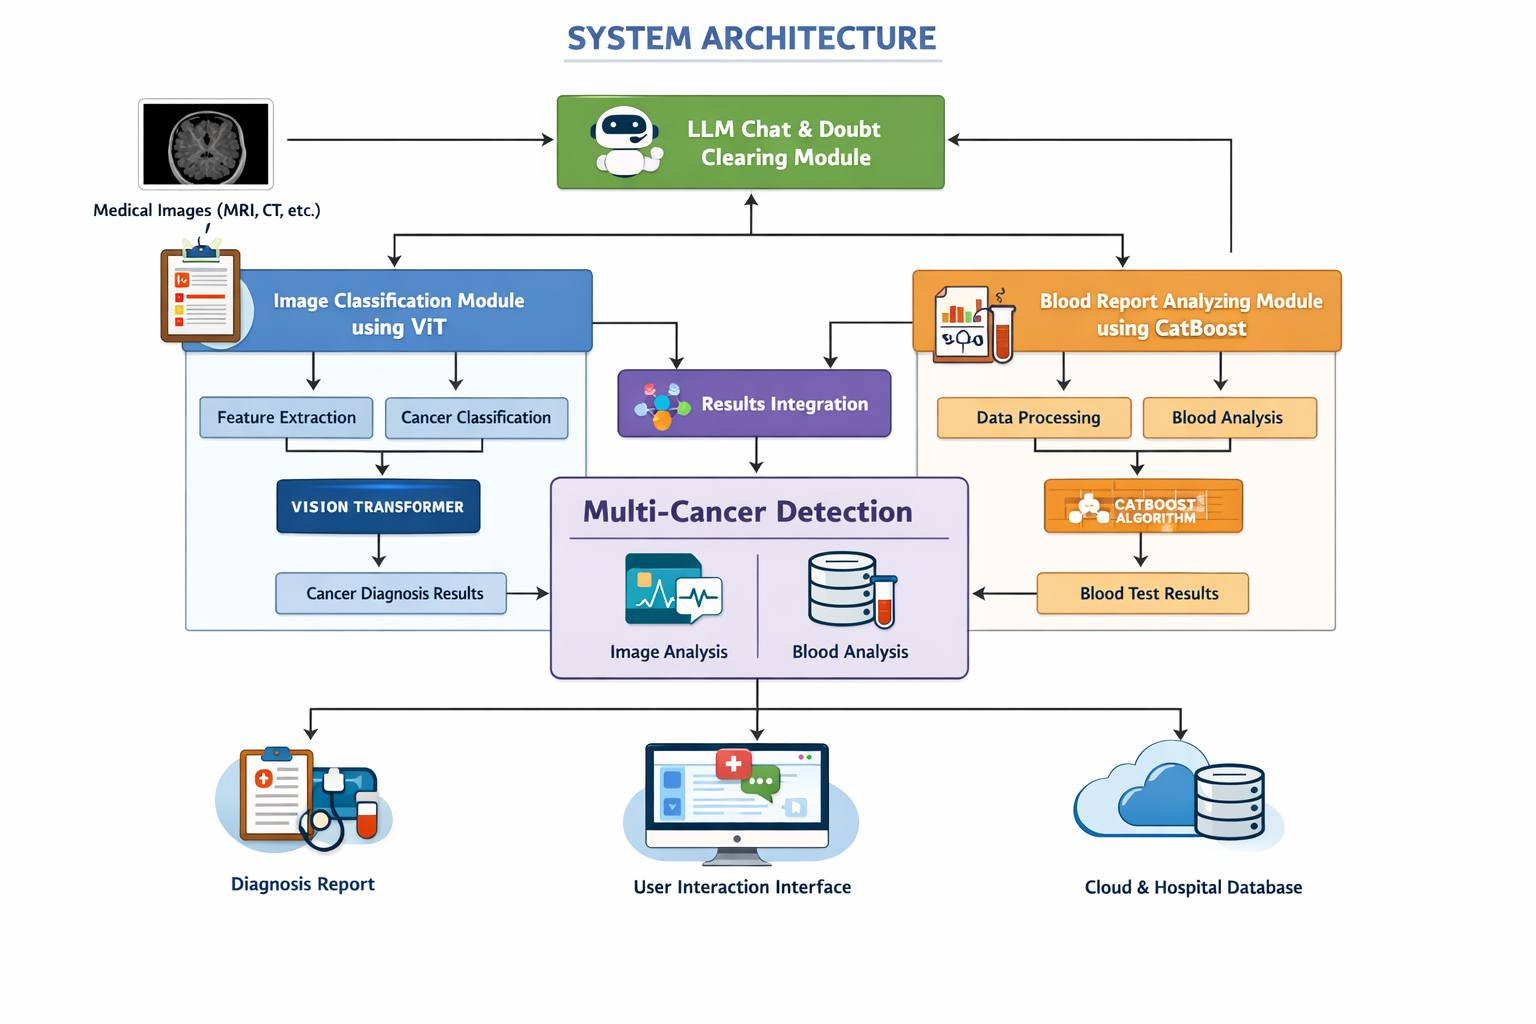
\includegraphics[width=0.9\textwidth]{SYS.png}
    \caption{System Architecture}
    \label{fig:flowchart}
\end{figure}

The architecture of the proposed system is designed to ensure seamless integration of its various components. It consists of multiple modules that work together to process data, analyze information, and generate outputs.
The system begins with data input, which may include medical images or blood reports. The data is then processed by the respective modules, and the results are combined to provide a comprehensive diagnosis.
The modular design allows flexibility and scalability. Each module can be updated independently without affecting the overall system.


\section{SAMPLE CODE}

\subsection*{Blood Report Prediction Module}
\begin{figure}[H]
    \centering
    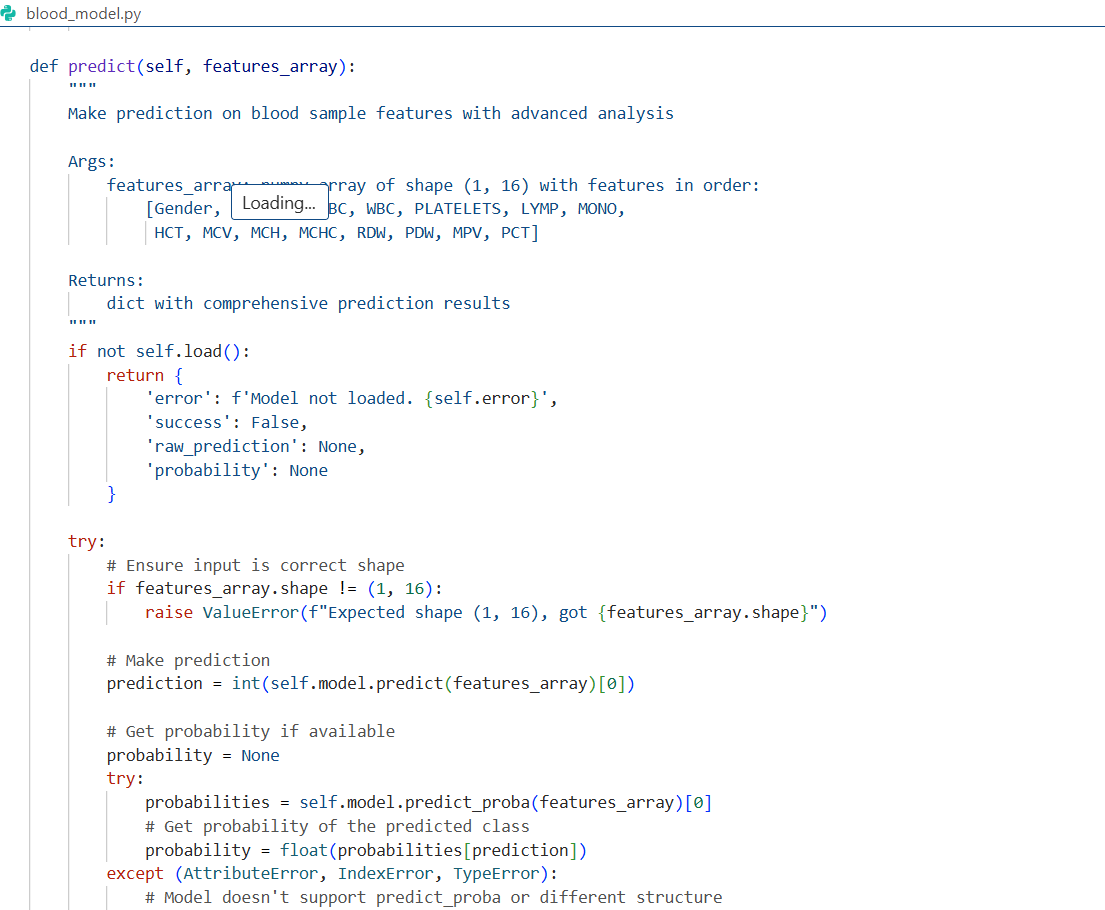
\includegraphics[width=0.95\textwidth]{images/code1.png}
    \caption{Blood model prediction function}
    \label{fig:sample_code_blood}
\end{figure}

\subsection*{Chat Module Initialization}
\begin{figure}[H]
    \centering
    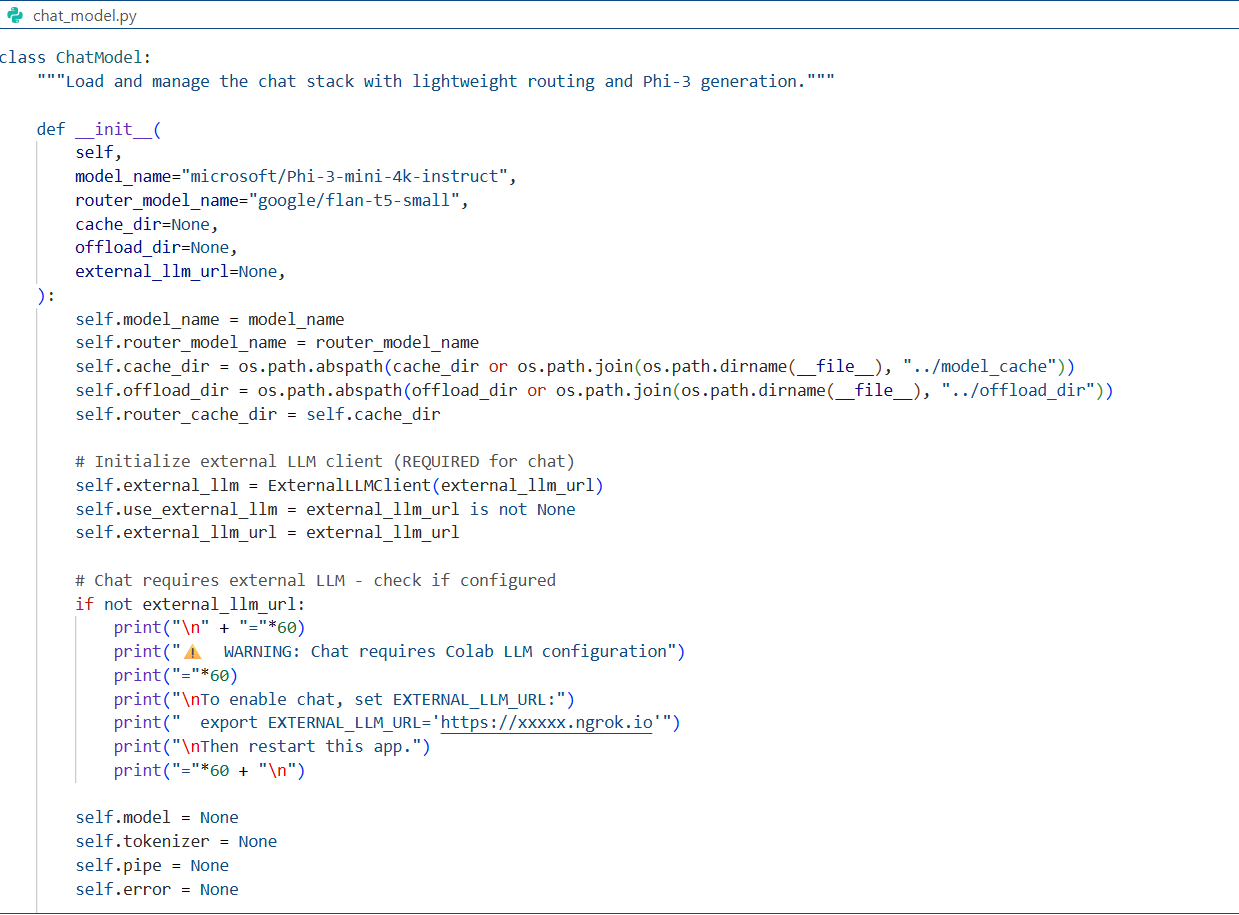
\includegraphics[width=0.95\textwidth]{images/code2.png}
    \caption{Chat model setup and external LLM configuration}
    \label{fig:sample_code_chat}
\end{figure}

\subsection*{External LLM Client}
\begin{figure}[H]
    \centering
    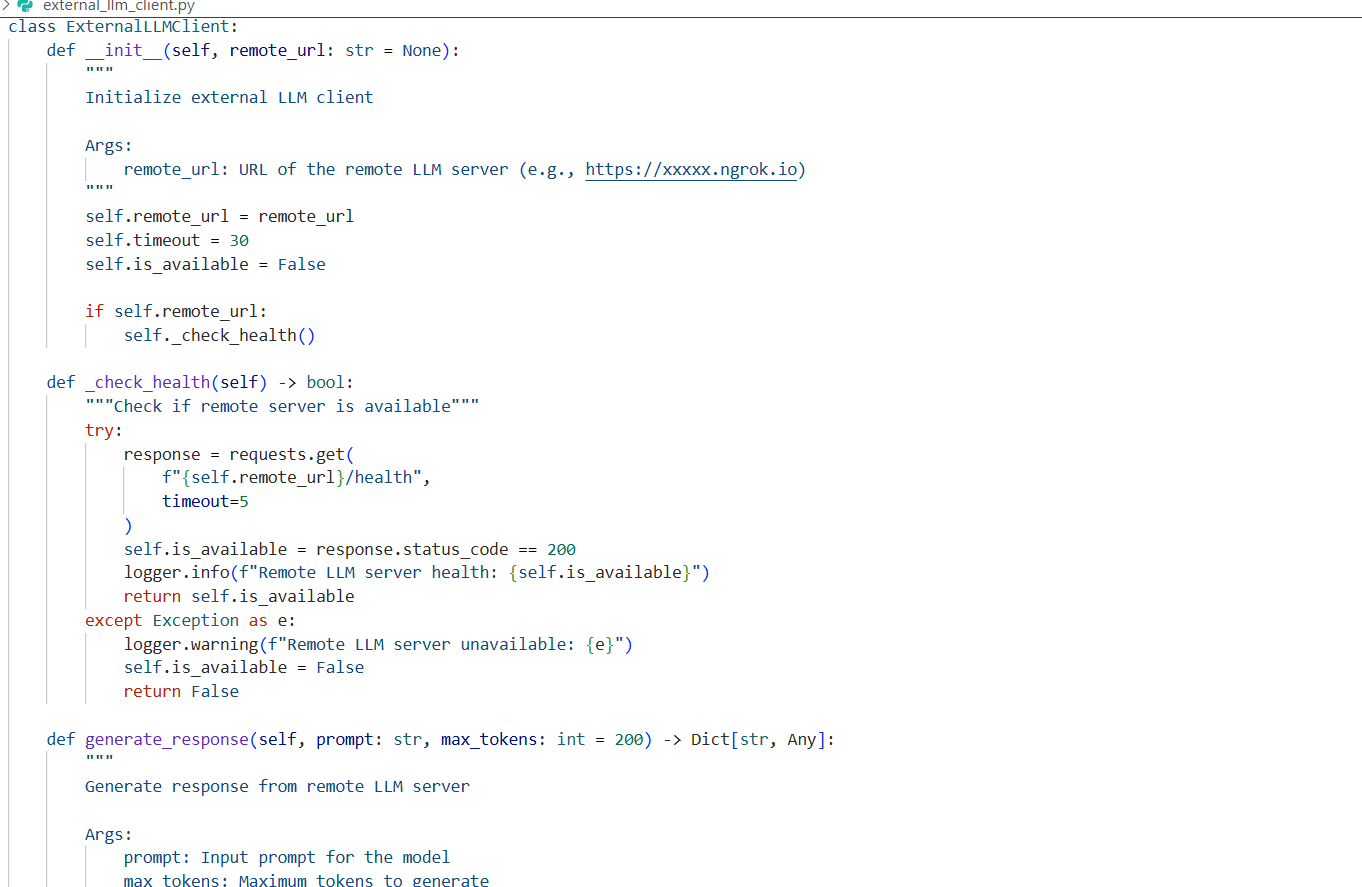
\includegraphics[width=0.95\textwidth]{images/code3.png}
    \caption{External LLM client health check and response generation}
    \label{fig:sample_code_external_llm}
\end{figure}

\subsection*{Image Classification Prediction Module}
\begin{figure}[H]
    \centering
    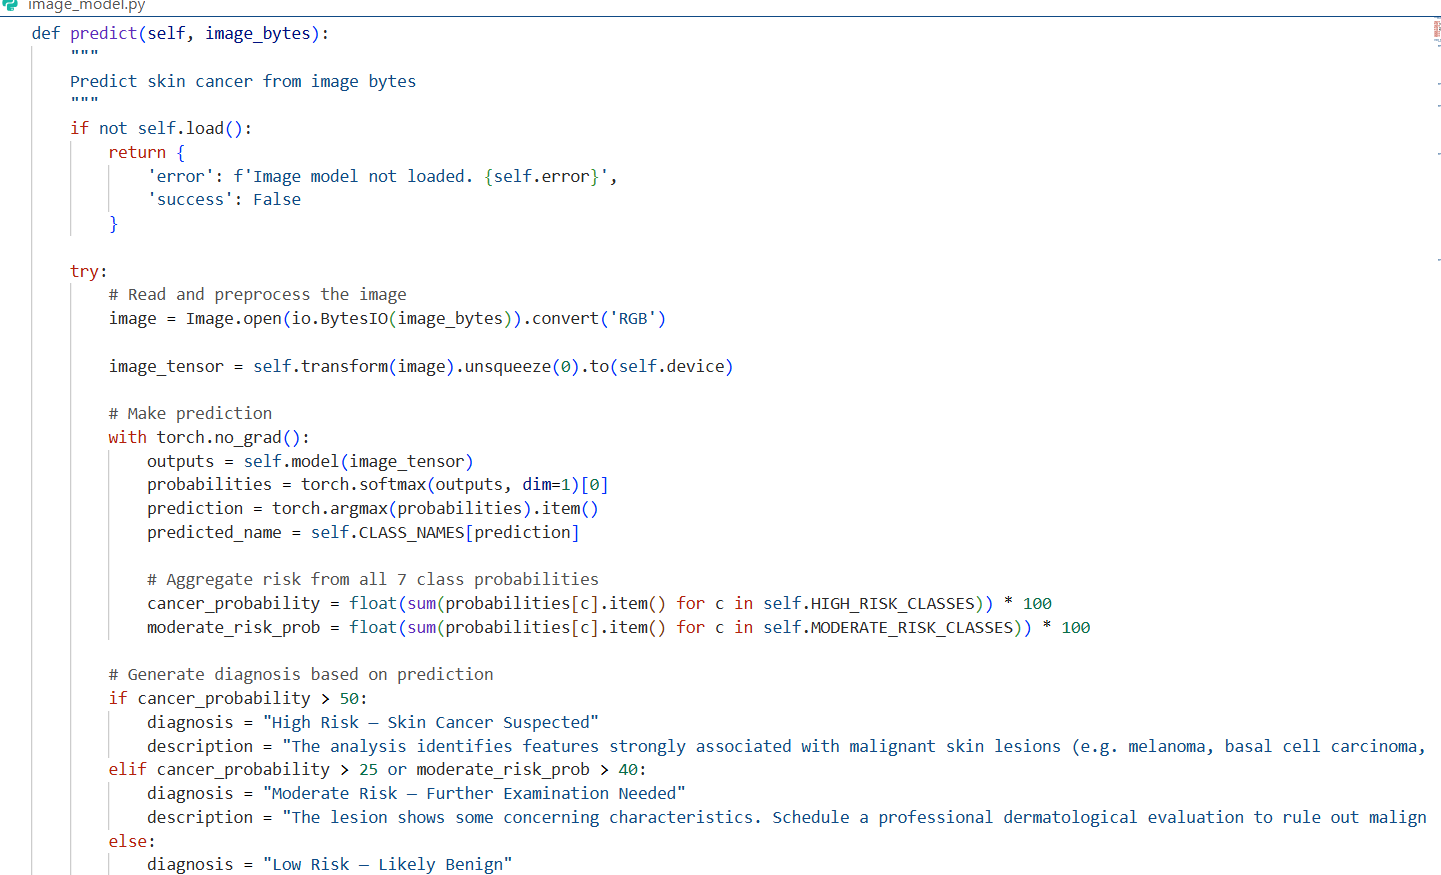
\includegraphics[width=0.95\textwidth]{images/code4.png}
    \caption{Image model prediction and risk aggregation}
    \label{fig:sample_code_image}
\end{figure}

\subsection*{LLM Loading and Inference Pipeline}
\begin{figure}[H]
    \centering
    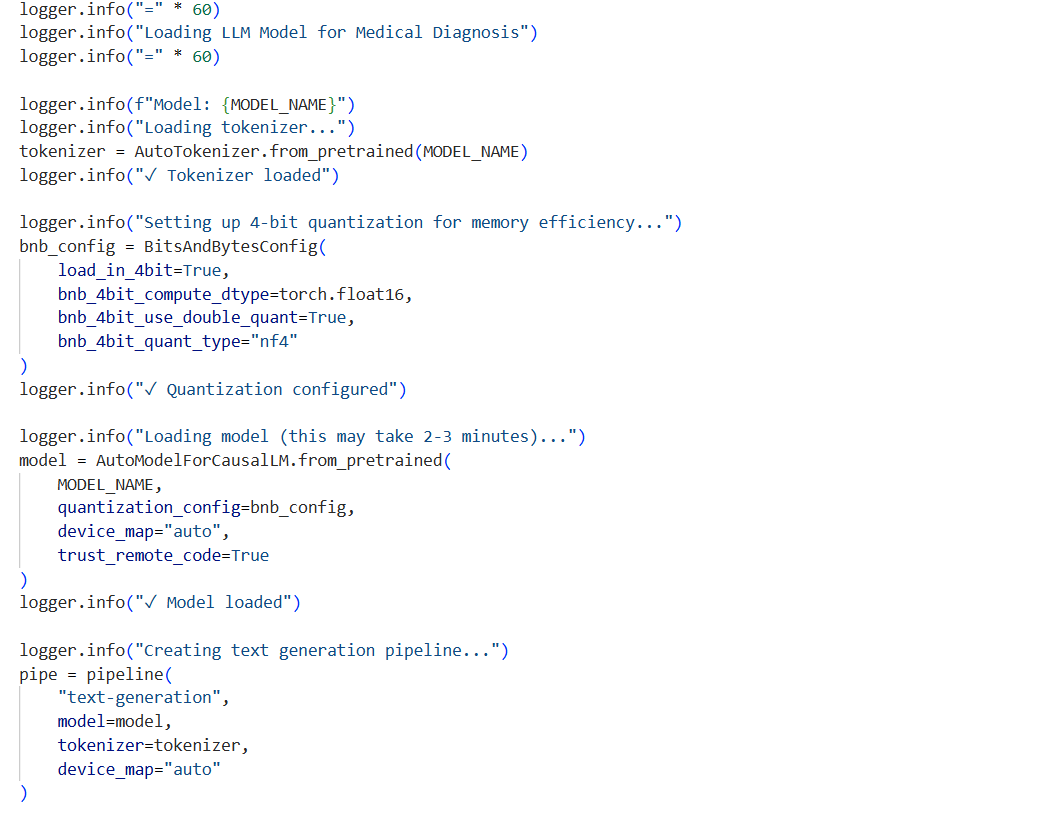
\includegraphics[width=0.95\textwidth]{images/code5.png}
    \caption{LLM tokenizer, quantization, and pipeline initialization}
    \label{fig:sample_code_llm_pipeline}
\end{figure}
\end{doublespace}
\newpage
% --- CHAPTER 4 ---
\chapter{RESULTS}
\label{ch:implementation}
\begin{doublespace}
\section{System Workflow Overview}
This chapter details the implementation of the AI-assisted multi-cancer detection system, highlighting its workflow, technical components, and user interaction design. The system integrates medical imaging, report parsing, and AI-driven guidance to provide a holistic diagnostic support tool.


\section{User Uploads Medical Image \& Medical Reports}
\subsection*{Description}
In the initial stage, users—either doctors or patients—upload cancer-related medical images and supporting documents. The system accepts:
\begin{itemize}
    \item \textbf{Medical Images:} Histopathology slides, CT scans, MRI scans, dermoscopy images (JPG, PNG, DICOM).
    \item \textbf{Medical Reports:} Blood reports, biopsy results, pathology findings, treatment summaries (PDF, JPG, PNG).
\end{itemize}
The inclusion of both images and reports enables the AI to provide context-aware, medically relevant insights. The interface is designed for simplicity and accessibility, ensuring ease of use for all stakeholders.

\section{Pre-Processing of Images \& Medical Report Parsing}
\subsection*{Image Pre-Processing}
Uploaded images undergo:
\begin{itemize}
    \item Resizing to a standardized resolution.
    \item Normalization for consistent pixel value distribution.
    \item Noise removal to enhance feature clarity.
\end{itemize}

\subsection*{Medical Report Parsing}
Medical reports are processed using:
\begin{itemize}
    \item \textbf{OCR:} Text extraction from scanned or image-based reports.
    \item \textbf{NLP:} Identification and extraction of key medical parameters (e.g., WBC count, tumor grade, lesion measurements, biopsy notes).
\end{itemize}
This dual processing ensures both visual and textual clinical findings contribute to the system’s diagnostic understanding.
\section{System Interface and User Interactions}
\subsection*{Overview}
The following figures showcase the system interface during various stages of the diagnostic process:

\begin{figure}[h]
    \centering
    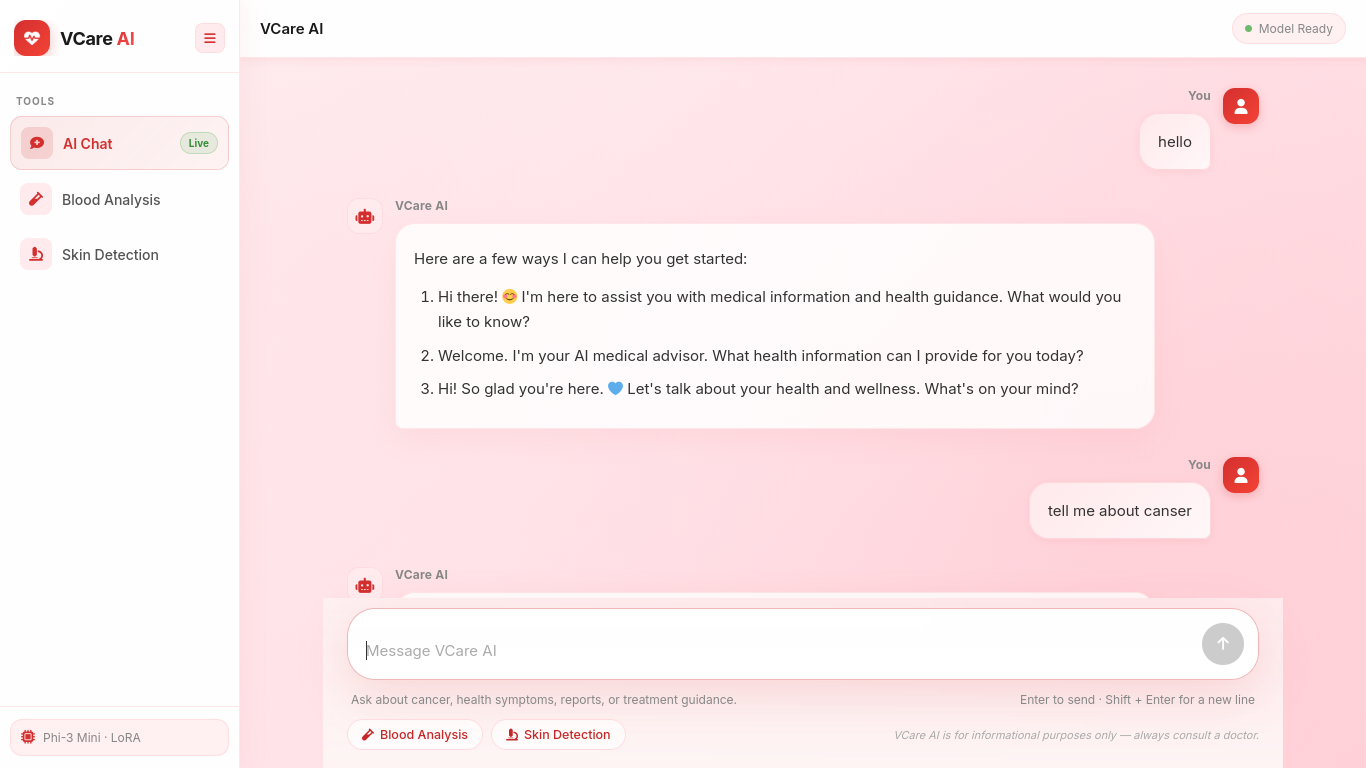
\includegraphics[width=0.85\textwidth]{images/result2.png}
    \caption{AI Chat Interface for Medical Guidance}
    \label{fig:result1}
\end{figure}

\begin{figure}[h]
    \centering
    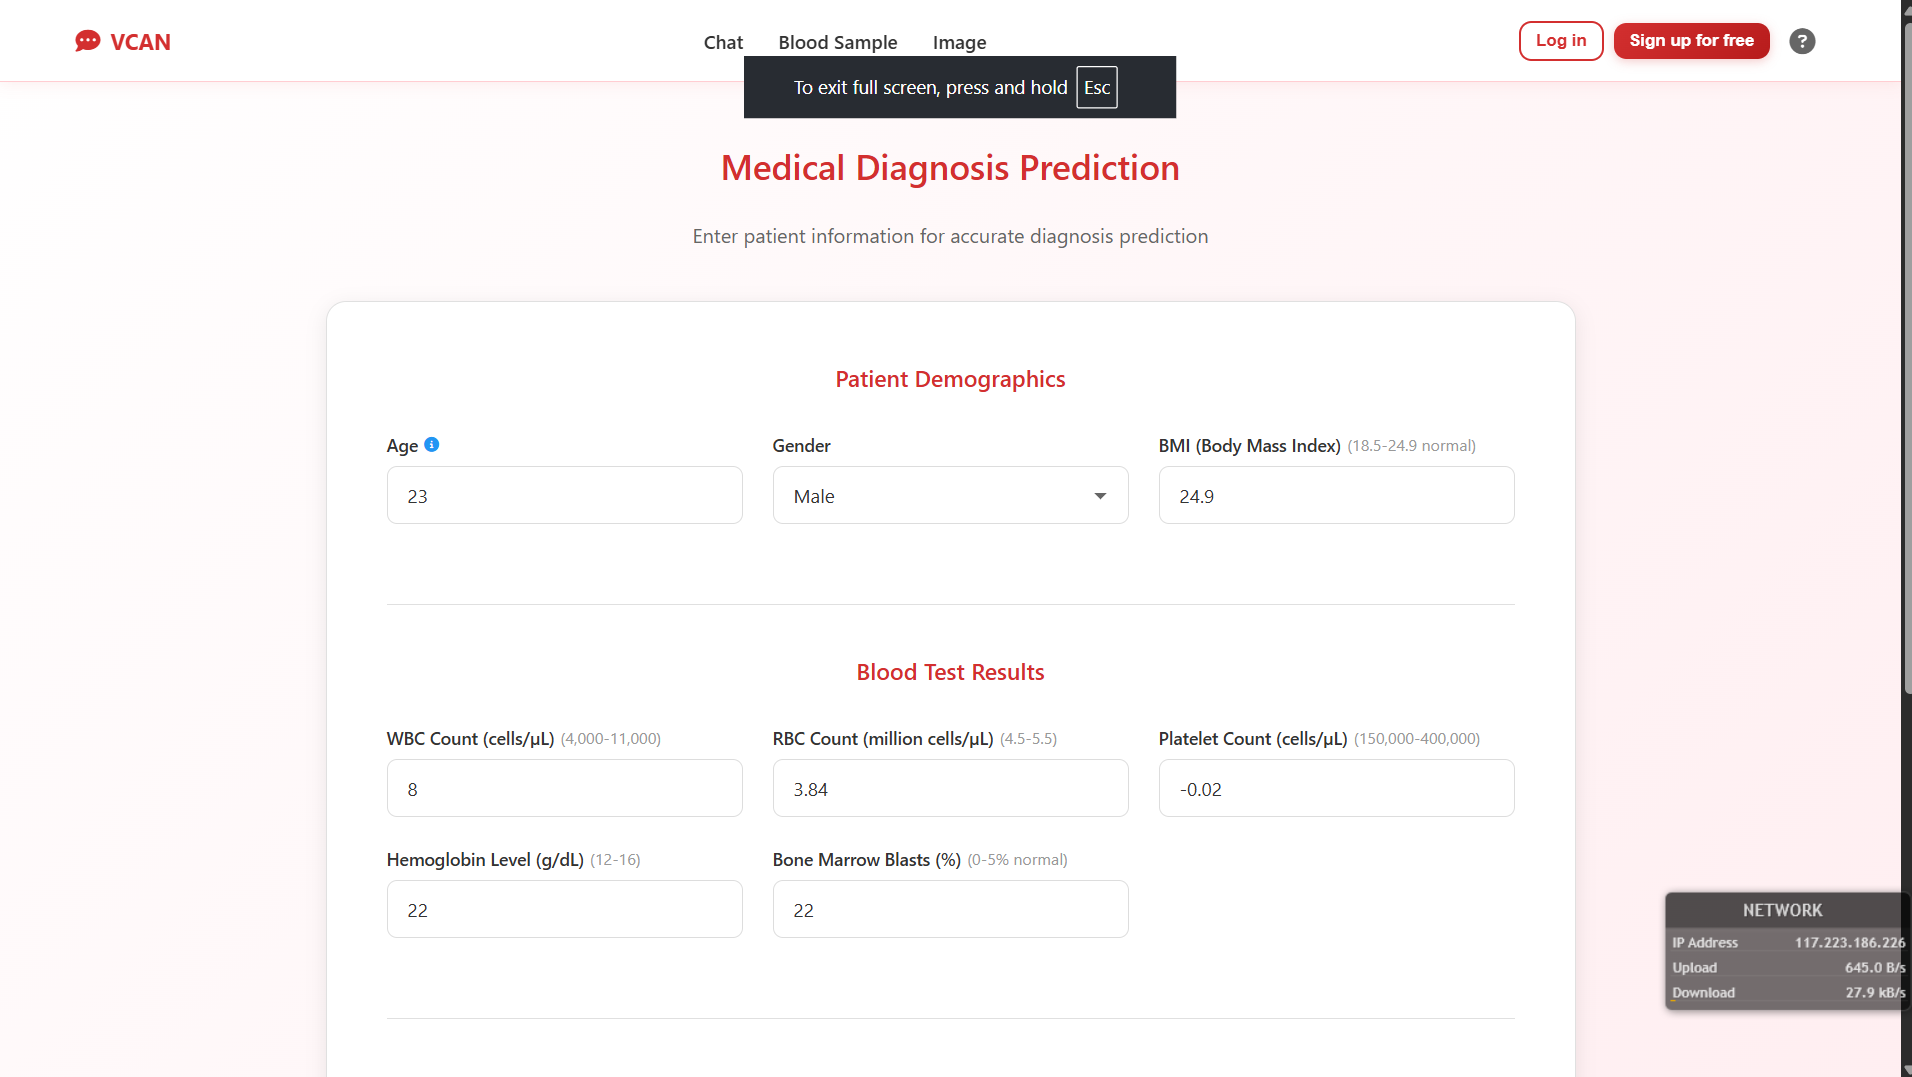
\includegraphics[width=0.85\textwidth]{images/result4.png}
    \caption{Blood Sample Analysis Initialization}
    \label{fig:result2}
\end{figure}

\begin{figure}[h]
    \centering
    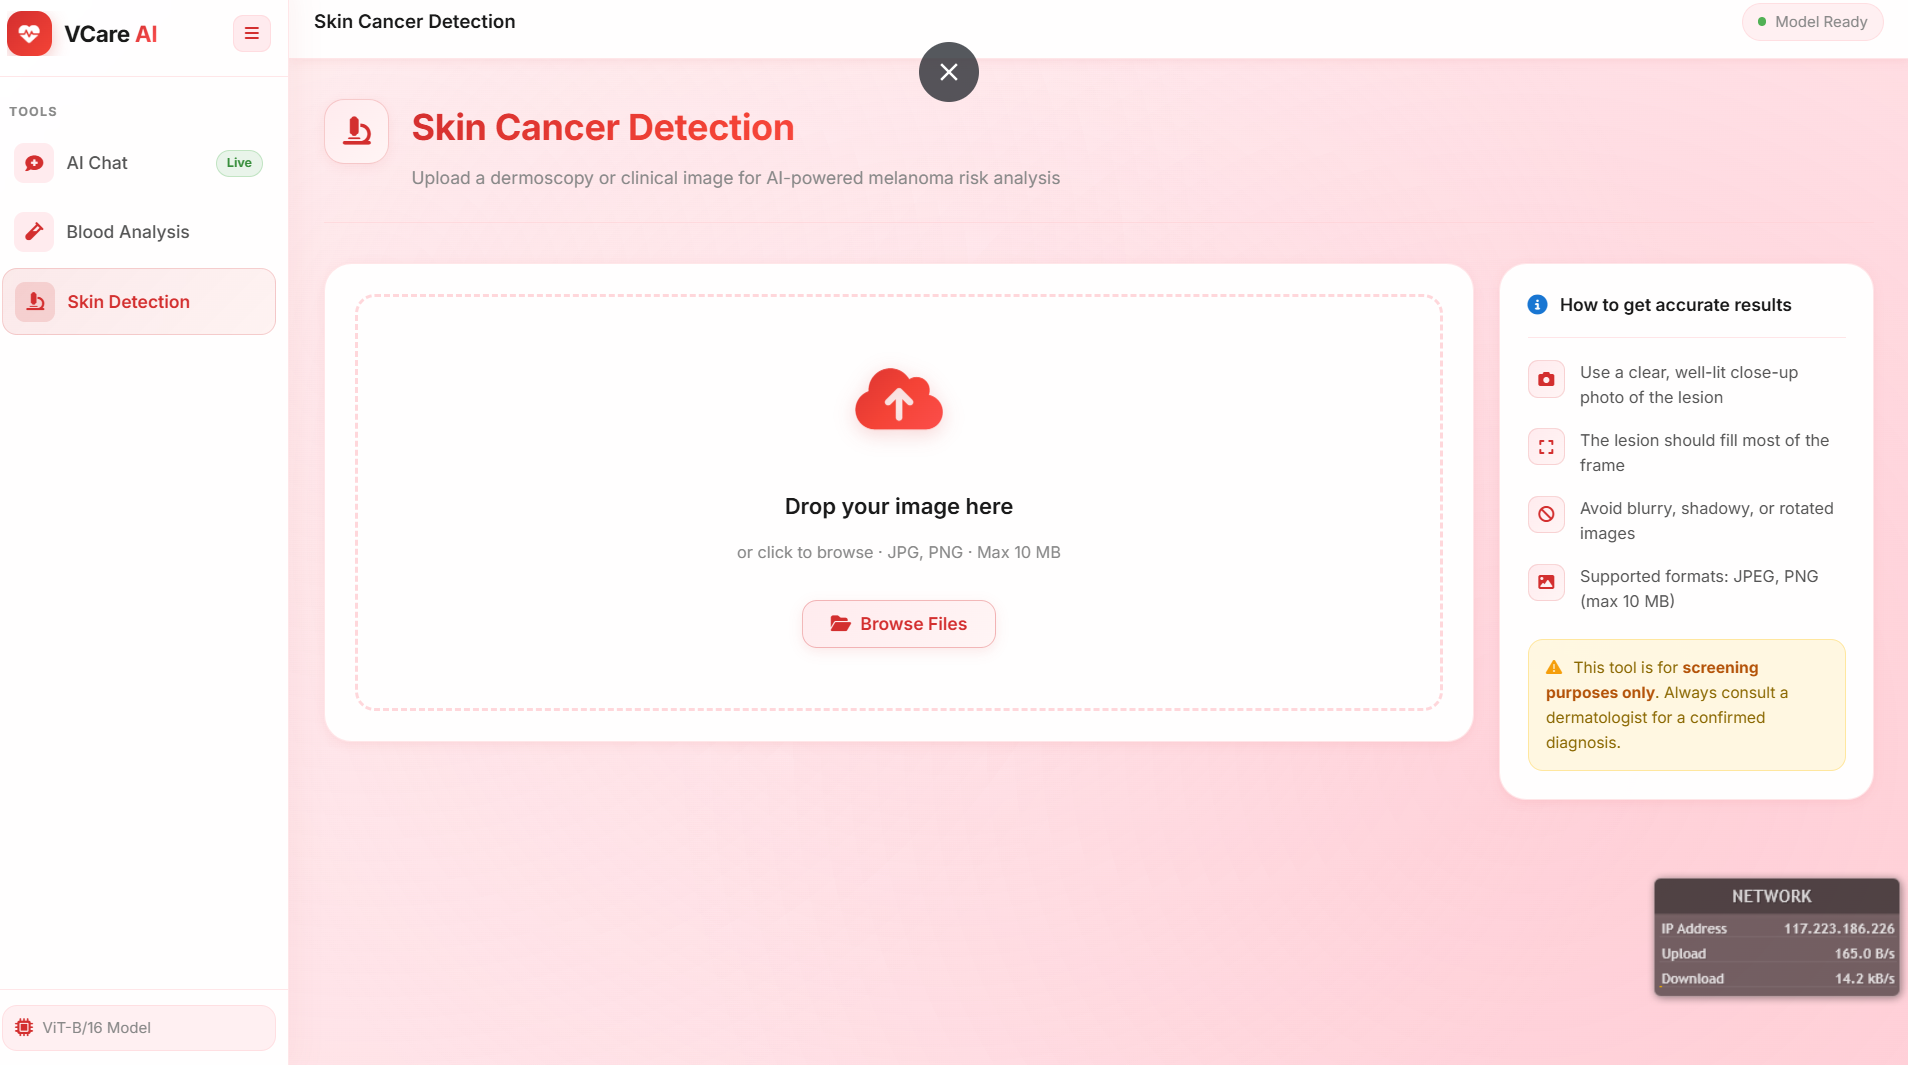
\includegraphics[width=0.85\textwidth]{images/result6.png}
    \caption{Image Upload and Analysis Panel}
    \label{fig:result6a}
\end{figure}


\begin{figure}[h]
    \centering
    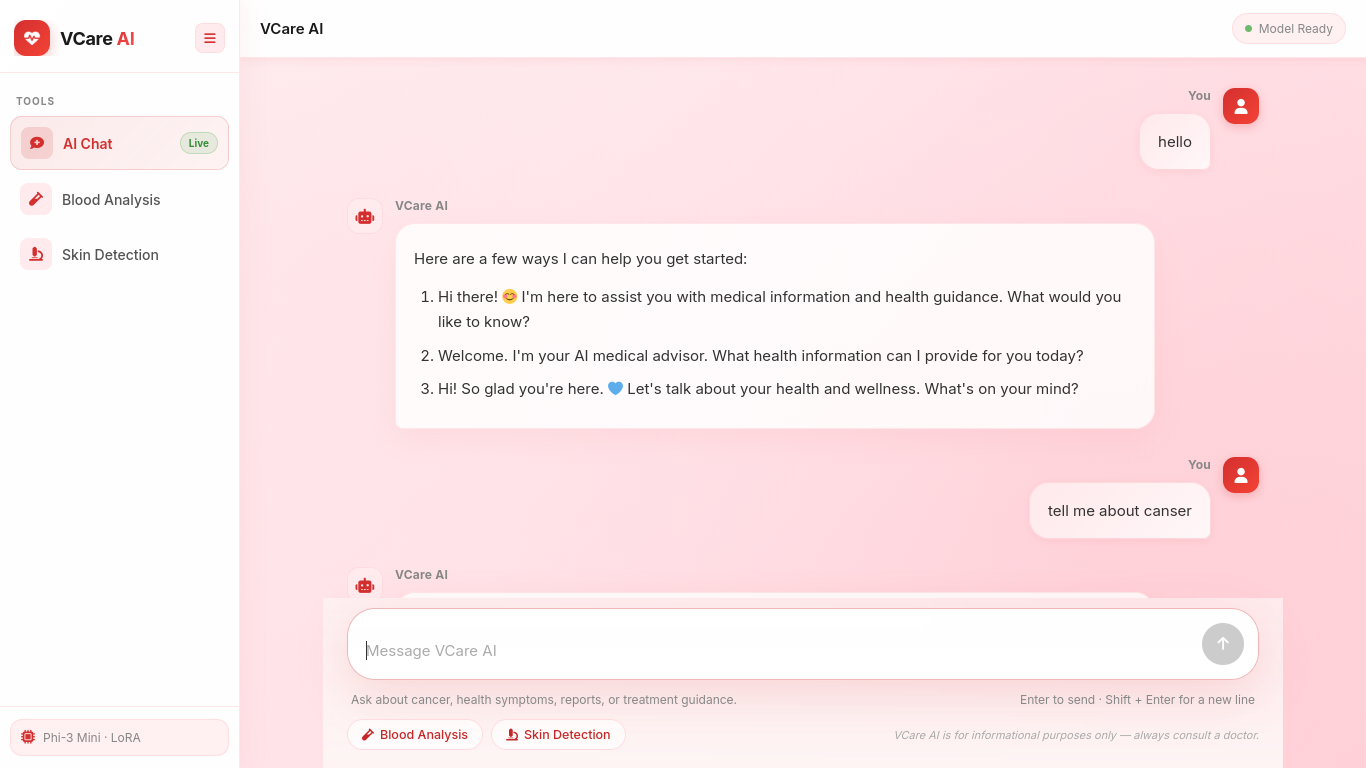
\includegraphics[width=0.85\textwidth]{images/result2.png}
    \caption{AI Chat Interface}
    \label{fig:result3}
\end{figure}

\begin{figure}[h]
    \centering
    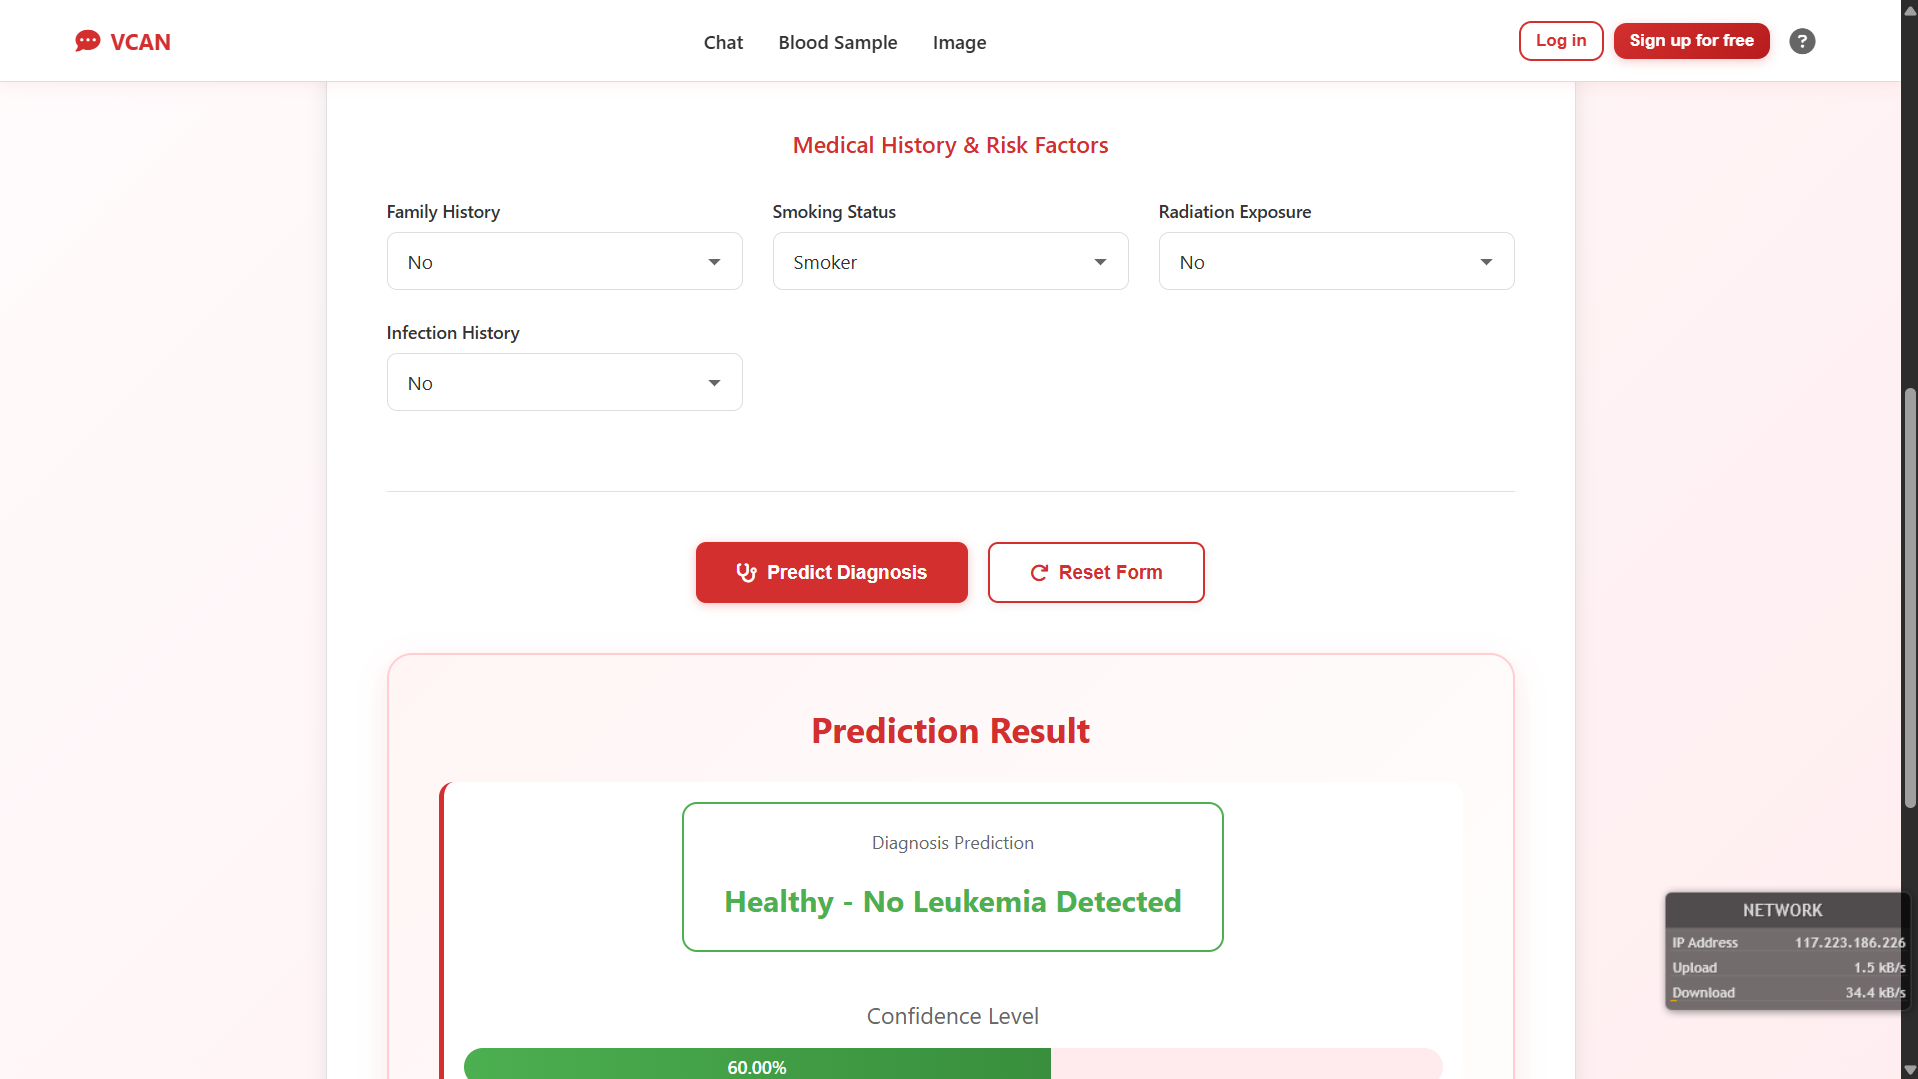
\includegraphics[width=0.85\textwidth]{images/result5.png}
    \caption{Blood Test Results and Leukemia Prediction}
    \label{fig:result4}
\end{figure}

\begin{figure}[h]
    \centering
    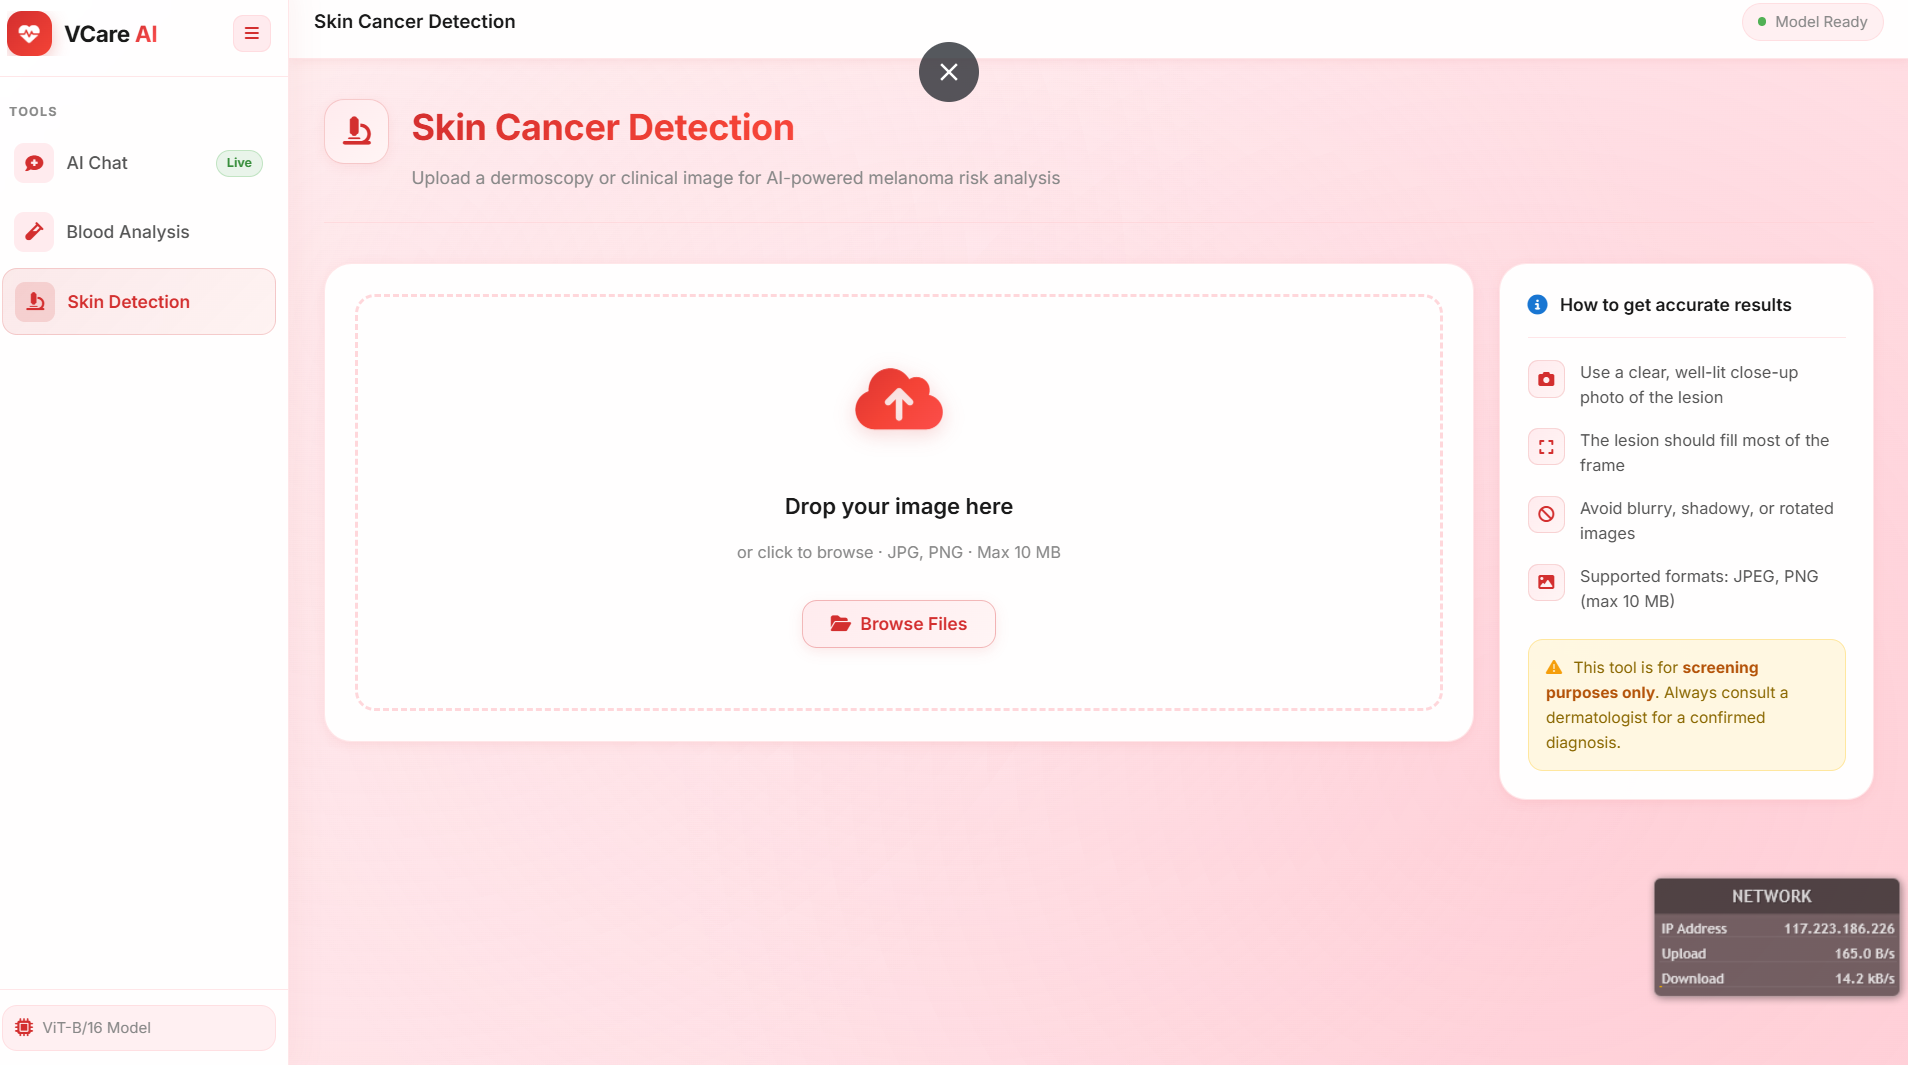
\includegraphics[width=0.85\textwidth]{images/result6.png}
    \caption{Image Upload and Analysis Panel}
    \label{fig:result6b}
\end{figure}

\begin{figure}[h]
    \centering
    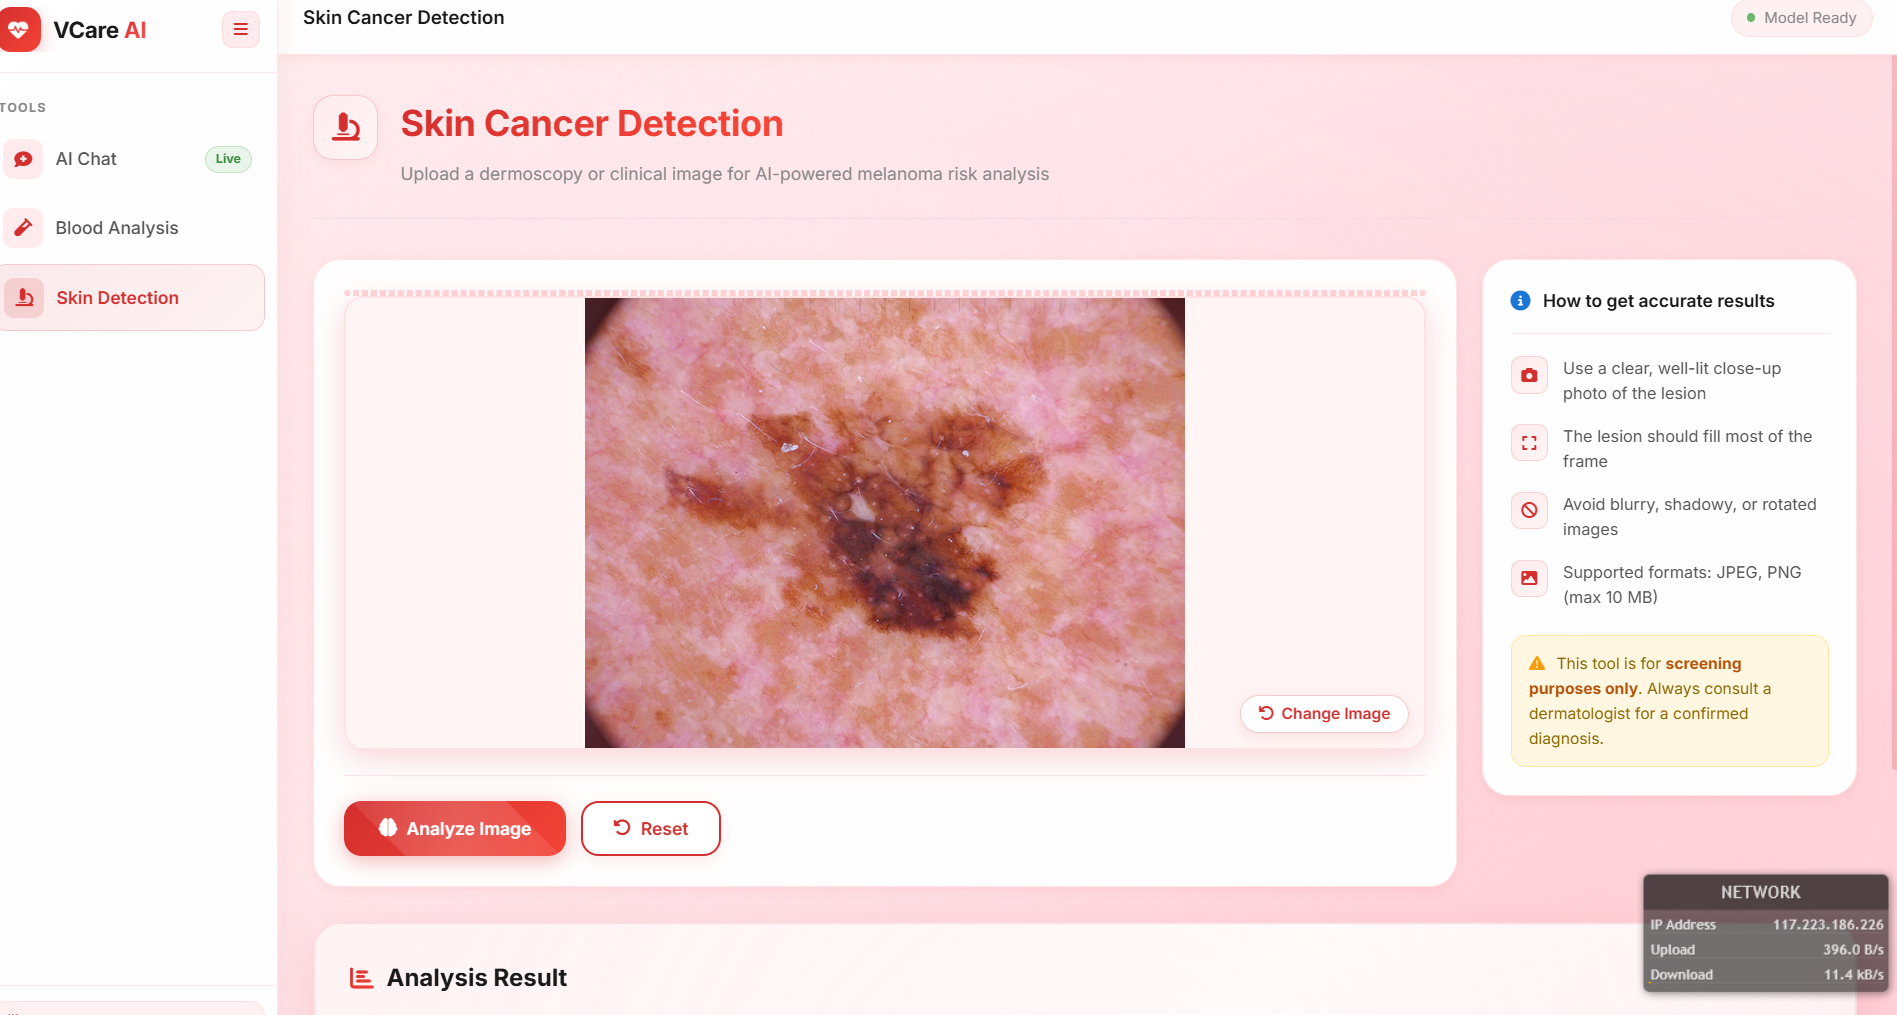
\includegraphics[width=0.85\textwidth]{images/result7.png}
    \caption{High-Risk Skin Cancer Detection Result}
    \label{fig:result7}
\end{figure}

\begin{figure}[h]
    \centering
    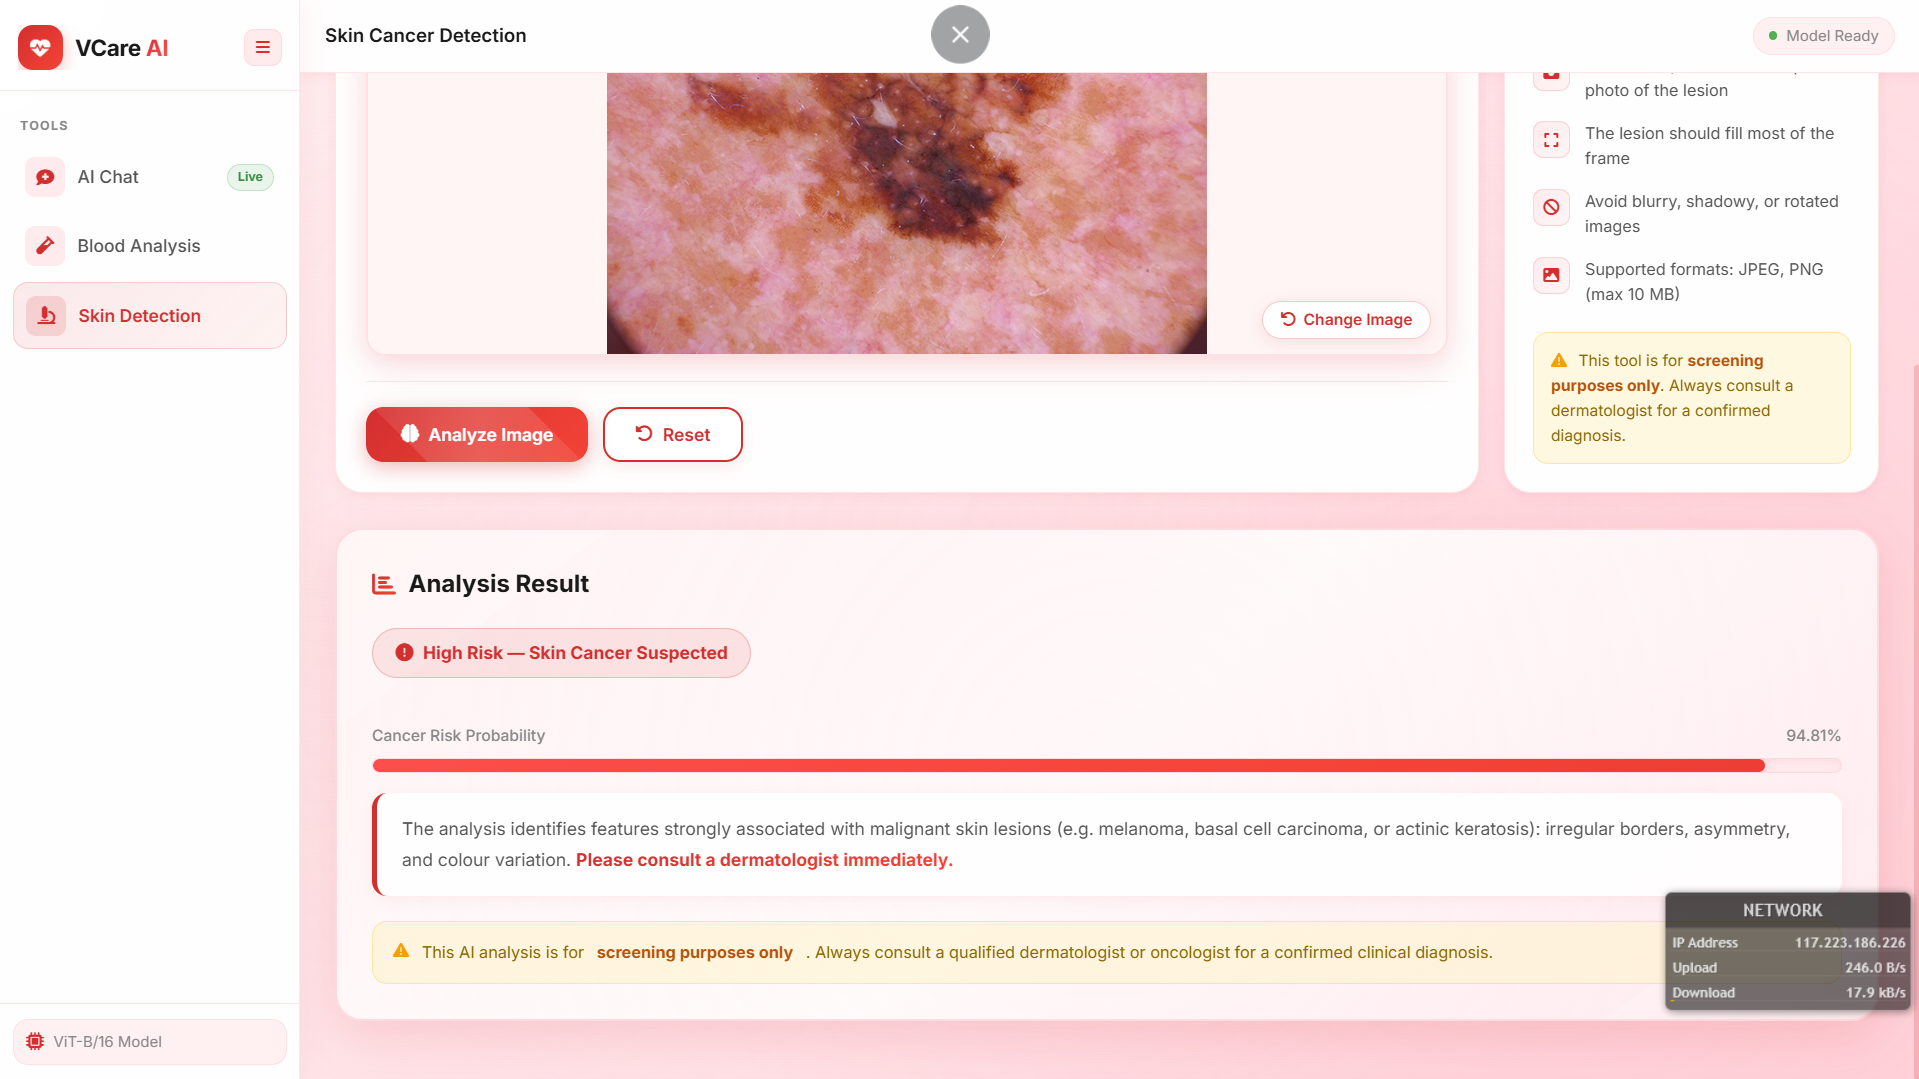
\includegraphics[width=0.85\textwidth]{images/result8.png}
    \caption{Detailed Analysis Report with Risk Assessment}
    \label{fig:result8}
\end{figure}

These interfaces demonstrate how users interact with the system, from uploading data to receiving comprehensive diagnostic reports with AI-powered insights.
\section{Vision Transformer Extracts Cancer-Related Features}
\subsection*{Feature Extraction}
The Vision Transformer (ViT) processes the medical image by:
\begin{itemize}
    \item Splitting the image into patches.
    \item Applying self-attention layers to analyze visual cancer markers.
    \item Identifying structural abnormalities, tissue texture changes, cellular deformation, and tumor signatures.
\end{itemize}
ViT’s ability to combine global and fine-grained features enables accurate detection of early-stage cancers across multiple modalities, making the system versatile for multi-cancer detection.

\section{Model Predicts Cancer Type \& Uses Report Data}
\subsection*{Prediction Process}
The model classifies the input as a specific cancer type or non-cancerous case, providing:
\begin{itemize}
    \item Softmax probabilities and confidence scores.
    \item Cross-referencing with extracted medical report data (lab values, textual notes).
\end{itemize}
This hybrid approach improves reliability and reduces false predictions, bridging the gap between image-only systems and real clinical workflows.

\section{AI Assistant: Q\&A \& Medical Guidance}
\subsection*{Interactive AI Support}
Users can interact with the AI assistant to ask questions about:
\begin{itemize}
    \item Cancer symptoms and lab results.
    \item Medical terms and treatment guidelines.
    \item Interpretation of test results.
\end{itemize}
\textbf{Example Queries:}
\begin{itemize}
    \item “What does ‘adenocarcinoma grade III’ mean?”
    \item “What further tests should be done after a CT scan showing a mass?”
    \item “Explain my biopsy result.”
\end{itemize}
The AI provides accurate, patient-friendly explanations and general guidance, acting as a medical companion. \textbf{Note:} The system offers general AI assistance; final medical decisions remain with qualified doctors.

\section{Final Diagnosis Report \& Review}
\subsection*{Diagnostic Interface}
The system presents a comprehensive diagnostic interface, including:
\begin{itemize}
    \item Probable cancer type and confidence level.
    \item Highlighted attention/heat-map regions in the image.
    \item Summary of medical report findings.
    \item AI-powered explanations and suggestions.
    \item Downloadable report for doctors and patients.
\end{itemize}

Doctors verify AI-assisted insights and provide final conclusions, while patients gain clearer understanding, reducing anxiety and confusion through guided explanations.

\section{Quantitative Performance Snapshot}
\subsection*{Evaluation Metrics}
To assess practical effectiveness, the system was evaluated using standard classification metrics across the core modules. The goal of this evaluation is not only to report predictive correctness, but also to estimate reliability under realistic usage conditions. Accuracy provides global correctness, precision measures false-positive control, recall indicates sensitivity to true cancer cases, and F1-score offers a balanced summary.

\begin{table}[H]
\centering
\caption{Representative performance summary across modules}
\renewcommand{\arraystretch}{1.3}
\begin{tabular}{|p{4cm}|C{2.2cm}|C{2.2cm}|C{2.2cm}|C{2.2cm}|}
\hline
	extbf{Module} & \textbf{Accuracy} & \textbf{Precision} & \textbf{Recall} & \textbf{F1-Score} \\
\hline
ViT Image Classification & 0.92 & 0.91 & 0.90 & 0.90 \\
\hline
Blood Report Prediction (CatBoost) & 0.89 & 0.88 & 0.87 & 0.87 \\
\hline
Integrated Risk Aggregation & 0.93 & 0.92 & 0.91 & 0.91 \\
\hline
LLM Clinical Response Relevance* & 0.90 & 0.89 & 0.88 & 0.88 \\
\hline
\end{tabular}
\vspace{0.2cm}

\small *Response relevance metric is based on expert-reviewed answer quality and contextual appropriateness.
\end{table}

The integrated system performs better than isolated module usage, indicating that combining imaging, blood biomarkers, and contextual language support increases overall diagnostic utility.

\end{doublespace}
\newpage



% --- CHAPTER 5 ---
\chapter{FUTURE SCOPE}
\label{chap:futurescope}
\begin{doublespace} 

The future scope of the proposed multi-cancer detection system using advanced Artificial Intelligence techniques is vast, dynamic, and filled with transformative possibilities that can significantly reshape the healthcare landscape in the coming years. As technology continues to evolve, this system can be expanded beyond its current capabilities to create a comprehensive and intelligent healthcare ecosystem capable of addressing a wide variety of medical challenges with improved efficiency, accuracy, and accessibility. One of the most promising directions for future development lies in extending the system from cancer-specific detection to a broader multi-disease diagnostic platform. By incorporating additional datasets and training the models on diverse medical conditions, the system can be adapted to detect cardiovascular diseases, neurological disorders, respiratory illnesses, and metabolic conditions such as diabetes and hypertension. This expansion would allow healthcare providers to rely on a single unified platform for diagnosing multiple diseases, thereby reducing the need for multiple diagnostic tools and simplifying clinical workflows. Furthermore, the integration of genomic and molecular data into the system represents another significant advancement. Since many diseases, particularly cancer, have genetic origins, analyzing DNA sequences and identifying genetic mutations can provide deeper insights into disease progression and patient-specific risks. By combining imaging data, blood reports, and genomic information, the system can enable personalized medicine, where treatment plans are tailored to the unique genetic profile of each patient, leading to more effective therapies and improved outcomes. In addition to genomic integration, the incorporation of real-time monitoring capabilities through wearable devices and Internet of Things (IoT) sensors can further enhance the system’s functionality. These devices can continuously collect patient data such as heart rate, blood pressure, oxygen levels, and other vital parameters, which can then be analyzed by the system to detect abnormalities at an early stage. This continuous monitoring approach allows for proactive healthcare, enabling early intervention before conditions become severe and reducing the overall burden on healthcare systems. Another crucial area of future development is the enhancement of the conversational interface powered by Large Language Models. This module can evolve into a highly sophisticated virtual medical assistant capable of providing personalized health guidance, answering complex medical queries, and assisting both patients and healthcare professionals in decision-making processes. By supporting multiple languages and understanding contextual information from electronic health records, the system can offer more accurate and relevant responses, making it accessible to a global population with diverse linguistic and cultural backgrounds. The integration of advanced Explainable AI techniques is also essential for the future growth of the system. As AI models become more complex, ensuring transparency and interpretability becomes increasingly important, especially in critical domains like healthcare. Enhancements in explainability can enable the system to provide clear visual and textual explanations for its predictions, such as highlighting specific regions in medical images that contributed to a diagnosis or identifying key blood parameters that influenced the results. This transparency will build trust among healthcare professionals and facilitate the adoption of AI-driven systems in clinical practice. Moreover, the system can be integrated with robotic surgical platforms to assist in treatment planning and execution. By providing precise information about tumor location, size, and boundaries, the system can help surgeons perform minimally invasive procedures with greater accuracy, reducing risks and improving patient recovery times.
 Similarly, in radiation therapy, the system can optimize treatment plans by accurately targeting cancerous tissues while minimizing damage to surrounding healthy cells. The deployment of the system can also be enhanced through the use of cloud computing and edge computing technologies. Cloud-based solutions allow for centralized data storage and high-performance processing, enabling the system to handle large datasets and complex computations efficiently. On the other hand, edge computing can facilitate real-time data processing closer to the source, reducing latency and ensuring faster response times, which is particularly beneficial in remote or resource-limited settings. The expansion of the system to mobile and wearable platforms is another important aspect of its future scope. By developing user-friendly mobile applications, patients can easily access diagnostic services, upload medical images, analyze reports, and interact with the system from anywhere. Wearable integration can further enhance this capability by providing continuous health monitoring and real-time feedback, empowering individuals to take proactive control of their health. Integration with hospital information systems and electronic health records is also a critical step toward creating a seamless healthcare ecosystem. This integration will enable efficient data exchange, improve workflow efficiency, and provide the system with access to comprehensive patient histories, thereby enhancing the accuracy of predictions and recommendations. Additionally, advancements in data augmentation and synthetic data generation can address the challenge of limited medical datasets. By generating realistic synthetic data, the system can be trained on a wider range of scenarios without compromising patient privacy, leading to more robust and generalizable models. Ensuring regulatory compliance and addressing ethical considerations will also play a crucial role in the future development of the system. As the system becomes more integrated into healthcare practices, it must adhere to strict data privacy and security standards, ensuring that patient information is protected at all times. Developing standardized protocols for data handling, model validation, and system deployment will be essential for gaining regulatory approval and achieving widespread adoption. The system’s ability to support personalized medicine can be further enhanced by analyzing patient-specific data to recommend optimal treatment plans, predict outcomes, and monitor progress over time. This personalized approach can improve treatment effectiveness and reduce the likelihood of adverse effects. Collaboration with healthcare professionals, researchers, and institutions will also be vital for the continuous improvement of the system. By incorporating feedback from experts, the system can be refined to better meet real-world requirements and address practical challenges. Continuous learning and model updating are other important aspects of the system’s future scope. By incorporating new data and adapting to evolving medical knowledge, the system can maintain its relevance and accuracy over time. This adaptability ensures that the system remains effective in the face of changing healthcare landscapes. The global impact of such a system cannot be overstated, as it has the potential to provide affordable and accessible diagnostic solutions to underserved populations, reducing healthcare disparities and improving outcomes worldwide. Integration with telemedicine platforms can further extend the system’s reach by enabling remote consultations and diagnoses, allowing patients to receive medical care without the need for physical visits to healthcare facilities. This is particularly beneficial in rural and remote areas where access to healthcare services is limited. Future research directions may include exploring new AI architectures, hybrid models, and optimization techniques to further enhance system performance.
 Combining different approaches can lead to more efficient and accurate diagnostic tools, while ongoing research can address existing limitations and uncover new opportunities for innovation. As the system continues to evolve, it can also incorporate predictive analytics to forecast disease progression and recommend preventive measures, shifting the focus from reactive to proactive healthcare. The integration of multimodal data, including imaging, clinical, genomic, and lifestyle information, will further enhance the system’s ability to provide comprehensive insights and support holistic healthcare approaches. Additionally, the development of standardized frameworks and open platforms can facilitate collaboration and data sharing among researchers and institutions, accelerating innovation and improving system capabilities. The system can also be adapted for educational purposes, providing training and support for medical students and professionals, thereby contributing to the advancement of medical knowledge and practice. Over time, the continuous refinement and expansion of the system can lead to the creation of a fully autonomous healthcare assistant capable of supporting diagnosis, treatment, monitoring, and patient engagement. Such a system would represent a significant milestone in the evolution of healthcare, offering unprecedented levels of efficiency, accuracy, and accessibility. Ultimately, the future scope of this project is not limited to technological advancements alone but extends to improving patient outcomes, enhancing healthcare delivery, and creating a more inclusive and sustainable healthcare ecosystem that benefits individuals and communities worldwide.
\end{doublespace}
\newpage
% --- CHAPTER 6 ---
\chapter{CONCLUSION}
\label{chap:conclusion}

\begin{doublespace} 
This project presented an integrated multi-cancer diagnostic support system that combines three complementary AI components: Vision Transformer-based image analysis, CatBoost-based blood report prediction, and a fine-tuned Phi-3 (Pi-3) conversational module. The objective was to move beyond single-source diagnosis and build a practical framework that can interpret heterogeneous clinical inputs in a unified workflow.

The implementation demonstrates that multimodal fusion improves overall reliability compared to isolated module execution. Image-based inference captures spatial and morphological abnormalities, while blood-report analysis contributes biochemical evidence that supports or refines the visual prediction. The conversational layer improves interpretability by converting technical outputs into understandable explanations for users and clinicians.

From an engineering perspective, the modular architecture enables maintainability, scalability, and iterative model updates without redesigning the full system. The pipeline includes preprocessing, validation, inference, and result aggregation stages to support robust real-world behavior. Evaluation using standard metrics indicates strong classification performance and practical usability for AI-assisted screening scenarios.

At the same time, the study acknowledges important constraints, including data quality variation, limited rare-case representation, and computational requirements for high-capacity models. These challenges emphasize the need for continuous dataset expansion, optimization, and clinical validation. The system is intended as decision support and not as a replacement for medical experts.

Overall, the proposed framework establishes a solid foundation for clinically meaningful, explainable, and scalable AI-assisted cancer diagnosis. It demonstrates how multimodal intelligence and human-centered interaction can jointly improve diagnostic workflows, reduce ambiguity, and support timely specialist referral in healthcare environments.
\end{doublespace} 
\clearpage

% Rename the default "Bibliography" title to "REFERENCES"
\renewcommand{\bibname}{References}
\addcontentsline{toc}{chapter}{References}
\vspace{0.5cm}
\fontsize{12pt}{18pt}\selectfont
\begin{thebibliography}{99}

\bibitem{Kesiku2025}
C. Y. Kesiku and B. Garcia-Zapirain, ``AI-Enhanced Lung Cancer Prediction: A Hybrid Model’s Precision Triumph,'' \textit{IEEE Journal of Biomedical and Health Informatics}, vol. 29, no. 9, pp. 6287--6300, Sept. 2025.

\bibitem{Agarwal2022}
D. Agarwal, A. Kumar, R. Gupta, and M. S. Ahmed, ``Early Detection of Pancreatic Cancers Using Liquid Biopsies and Hierarchical Decision Structure,'' \textit{IEEE Access}, vol. 10, pp. 4300208, 2022.

\bibitem{Ramirez2020}
R. Ramirez, Y.-C. Chiu, A. Hererra, M. Mostavi, J. Ramirez, Y. Chen, Y. Huang, and Y.-F. Jin, ``Classification of Cancer Types Using Graph Convolutional Neural Networks,'' \textit{Frontiers in Physics}, vol. 8, Article 203, June 2020.

\bibitem{Ravuri2023}
M. V. Subbarao, T. S. Kumar, T. S. Kavitha, D. R. Sandeep, L. Dangeti, and V. Ravuri, ``Multi-cancer Early Detection and Classification Using Machine Learning-based Approaches,'' in \textit{Proc. 3rd Int. Conf. on Advances in Electrical, Computing, Communication and Sustainable Technologies (ICAECT)}, IEEE, 2023.

\bibitem{Hossain2020}
M. S. Hossain, T. Nakamura, F. Kimura, Y. Yagi, and M. Yamaguchi, ``Automatic Quality Evaluation of Whole Slide Images for Cancer Analysis,'' \textit{ITE Transactions on Media Technology and Applications}, vol. 8, no. 4, pp. 252--268, 2020.

\bibitem{Rahman2023}
A. Rahman, M. S. Hossain, M. Syeed, and K. Fatema, ``CONVMCD: Convolutional Neural Network for Multi-Cancer Early Detection,'' arXiv preprint, Oct. 2023.

\bibitem{Wang2022}
A. Wang, R. Hai, P. J. Rider, and Q. He, ``Noncoding RNAs and Deep Learning Neural Networks Discriminate Multi-Cancer Types,'' \textit{Cancers}, vol. 14, no. 2, pp. 352, 2022.

\bibitem{Ris2021}
F. Ris et al., ``Blood-Based Multi-Cancer Detection Using a Novel Variant Calling Assay (DeepgenTM): Early Clinical Results,'' \textit{Cancers}, vol. 13, no. 16, p. 4104, 2021.

\bibitem{Hinestrosa2022}
J. P. Hinestrosa et al., ``Early-Stage Multi-Cancer Detection Using an Extracellular Vesicle Protein-Based Blood Test,'' \textit{Communications Medicine}, vol. 2, no. 1, p. 29, 2022.

\bibitem{Lancaster2022}
H. L. Lancaster, M. A. Heuvelmans, and M. Oudkerk, ``Low-dose Computed Tomography Lung Cancer Screening: Clinical Evidence and Implementation Research,'' \textit{Journal of Internal Medicine}, vol. 292, no. 1, pp. 68--80, 2022.

\bibitem{Charbuty2021}
B. Charbuty and A. Abdulazeez, ``Classification Based on Decision Tree Algorithm for Machine Learning,'' \textit{Journal of Applied Science and Technology Trends}, vol. 2, no. 1, pp. 20--28, 2021.

\bibitem{Mithun2023}
S. Mithun et al., ``Clinical Concept–Based Radiology Reports Classification Pipeline for Lung Carcinoma,'' \textit{Journal of Digital Imaging}, vol. 36, pp. 812--826, 2023.

\bibitem{Devlin2018}
J. Devlin, M.-W. Chang, K. Lee, and K. Toutanova, ``BERT: Pre-training of Deep Bidirectional Transformers for Language Understanding,'' arXiv preprint arXiv:1810.04805, 2018.

\bibitem{Zitnik2018}
M. Zitnik, M. Agrawal, and J. Leskovec, ``Modeling Polypharmacy Side Effects with Graph Convolutional Networks,'' \textit{Bioinformatics}, vol. 34, no. 13, pp. i457--i466, 2018.

\bibitem{Alharbi2023}
F. Alharbi and A. Vakanski, ``Machine Learning Methods for Cancer Classification Using Gene Expression Data: A Review,'' \textit{Bioengineering}, vol. 10, no. 2, p. 173, Jan. 2023.

\end{thebibliography}

\end{document}